% IEEE Transactions on Medical Imaging — MIC (IEEE TMI submission)
% Compile: pdflatex -> bibtex -> pdflatex -> pdflatex
\documentclass[journal]{IEEEtran}

% ---- Math / fonts ----
\usepackage{amsmath}
\usepackage{amssymb}
% Times Roman text + math with TU encoding shapes (bold/italic/bold-italic
% available under XeTeX/Tectonic, not just T1/pdflatex). Without this,
% IEEEtran's default Adobe Times (ptm) has no TU font definition file,
% so \textbf / \emph / \textit silently fall back to upright Latin Modern.
\usepackage{newtxtext,newtxmath}

% ---- Graphics / tables ----
\usepackage{graphicx}
\usepackage{booktabs}
\usepackage{array}
\usepackage{multirow}

% ---- Utilities ----
\usepackage{xcolor}
\usepackage{url}
\usepackage{hyperref}
\usepackage{microtype}
\usepackage{listings}
\usepackage{algorithm}
\usepackage{algpseudocode}
\usepackage{caption}
\usepackage{subcaption}
\usepackage{cite}

\hypersetup{
  colorlinks=true,
  linkcolor=blue!70!black,
  citecolor=green!50!black,
  urlcolor=blue!70!black,
}

\lstset{
  basicstyle=\ttfamily\small,
  breaklines=true,
  columns=fullflexible,
}

% --------------------------------------------------
\title{A 16-Bit-Native Entropy Coding Pipeline for\\
       Lossless Medical Image Compression}

\author{Kuldeep~Singh%
\thanks{K.\ Singh is with Innovaccer Inc.
E-mail: kuldeep.singh@innovaccer.com.
ORCID: 0009-0004-8476-0118.
Code: \url{https://github.com/pappuks/medical-image-codec}.}%
}


% --------------------------------------------------

\begin{document}
\maketitle

% ============================================================
\begin{abstract}
Lossless compression is essential in medical imaging, where archival storage
and diagnostic workflows require exact pixel reconstruction from
10--16-bit-per-sample data. Most entropy coders target 8-bit byte streams;
medical images break this assumption by producing residual alphabets of
thousands of symbols after spatial prediction. This paper presents MIC, a
lossless codec for Digital Imaging and Communications in Medicine (DICOM)
images that operates natively on 16-bit residuals. MIC combines spatial
prediction, 16-bit run-length encoding, and large-alphabet Finite State
Entropy (FSE), a table-driven implementation of asymmetric numeral systems
(ANS). Rather than splitting 16-bit pixels into byte pairs before entropy
coding, MIC treats each predicted residual as a single 16-bit symbol,
capturing correlations between the high and low byte directly---a structural
advantage quantified at 0.3--1.1 bits per symbol on the test dataset. The
implementation extends FSE to support up to 65,535-symbol alphabets and
includes a multi-state interleaved decoder that exploits
instruction-level parallelism (ILP) during decompression. Evaluation on 21
de-identified DICOM images spanning nine modalities shows the 16-bit-native
pipeline improves compression ratio by 5--22\% (geometric mean 14\%) over a
Delta+Zstandard baseline, reaching a geometric-mean ratio of 3.12
times---within 1\% of High-Throughput JPEG 2000 (HTJ2K, 3.15 times). A
multi-state interleaved decoder yields a 46\% geometric-mean FSE-stage
decompression speedup on ARM64 at four states and a further 7\% at
eight states. Single-threaded, MIC's C decoder is faster than HTJ2K on
every ARM64 image and on every AMD64 image we tested; a strip-parallel
mode adds
near-linear scaling for large images. A 20-kilobyte pure JavaScript
decoder and a Go WebAssembly build enable client-side in-browser
decoding, confirming that 16-bit-native entropy coding is a practical design
point where throughput, simplicity, and deployment portability matter.
\end{abstract}

\begin{IEEEkeywords}
medical image compression, lossless compression, entropy coding, asymmetric
numeral systems (ANS), finite state entropy (FSE), DICOM, high-bit-depth
imaging.
\end{IEEEkeywords}

% ============================================================
\section{Introduction}
\label{sec:intro}

\IEEEPARstart{M}{edical} imaging systems routinely generate large volumes of
high-bit-depth data. Modalities such as computed tomography (CT), magnetic
resonance imaging (MR), digital radiography (computed radiography,
CR; plain X-ray, XR), mammography, and tomosynthesis commonly store pixel
values at 10, 12, or 16 bits per sample. A single digital breast tomosynthesis
(DBT) acquisition view produces 60 or more reconstructed slices, totalling over
600\,MB of raw pixel data per view. A complete bilateral four-view screening
study exceeds 2\,GB uncompressed. Efficient lossless compression is essential
for archival storage, network transmission, and real-time rendering in clinical
Picture Archiving and Communication Systems (PACS) and diagnostic viewers.

DICOM~\cite{dicom} supports several established lossless transfer syntaxes,
including JPEG~2000, HTJ2K, JPEG-LS (a lossless/near-lossless predictive
standard), and Run-Length Encoding (RLE) Lossless. These methods offer
different tradeoffs among compression ratio, decoding speed, and
implementation complexity~\cite{liu2017,clunie2000}. JPEG~2000 and HTJ2K
provide strong compression performance but rely on transform and block-coding
pipelines that are comparatively complex. JPEG-LS uses predictive coding and
often yields strong lossless ratios, but its throughput characteristics remain
application-dependent. RLE Lossless is simple but typically provides limited
compression because it operates on byte-oriented runs and does not include an
effective decorrelation stage.

This work studies a different design point for lossless medical image
compression: direct coding of \textbf{predicted 16-bit residual streams}.
Throughout this paper, a \emph{residual stream} denotes the sequence of
per-pixel prediction errors $r_{i,j} = x_{i,j} - \hat{x}_{i,j}$ produced by a
spatial predictor, kept at the native 16-bit precision of the source pixels
rather than re-serialised into bytes. As a concrete example: if the predicted
pixel value is 1020 and the true pixel is 1023, the residual is $+3$.
Smooth regions therefore produce many residuals near zero, and these near-zero
residuals recur frequently---properties that motivate a 16-bit-native
run-length and entropy coding stage.

The central observation is that the dominant entropy coders in modern
compression systems, including Huffman coding, arithmetic coding, Lempel-Ziv
1977 (LZ77), and FSE/ANS as used in Zstandard, were designed primarily for
8-bit byte streams. Medical images break this assumption: DICOM stores pixels
at 10--16 bits per sample, yielding symbol alphabets of 1,024 to 65,536
entries. Even after spatial delta prediction, the residual alphabet for a
16-bit CT image can span tens of thousands of distinct values. An entropy coder
that assumes an 8-bit alphabet must either re-encode 16-bit symbols as byte
pairs (losing inter-byte correlation and doubling the number of coding steps)
or truncate the alphabet at 256 and fall back to raw storage for rare symbols.
This mismatch is structurally costly: for example, small signed residuals such
as $-2, -1, 0, +1$ have highly predictable high bytes, so encoding the high
and low bytes independently forces the coder to spend bits on information
already implied by the other byte. On our test images, the mutual information
$I(X_H;\,X_L)$ between the high and low bytes of delta residuals ranges from
0.3\,bits/symbol (MR) to 1.1\,bits/symbol (MG3), corresponding to 8--22\% of
total entropy and explaining MIC's 5--22\% empirical advantage over
Delta\,+\,Zstandard.

Based on this observation, we present MIC, a lossless codec that combines:
\begin{enumerate}
  \item a simple spatial predictor,
  \item a 16-bit-native run-length representation of the residual stream, and
  \item an extended FSE/tANS (table-based ANS) entropy coder supporting large
  active symbol alphabets.
\end{enumerate}

The codec also includes multi-state interleaved entropy decoding to improve
decompression throughput by increasing ILP.

\subsection{Contributions}

The main contributions of this paper are as follows.

\begin{enumerate}
  \item \textbf{A 16-bit-native lossless coding pipeline for medical images.}
  We present a Delta\,+\,16-bit RLE\,+\,extended FSE pipeline for grayscale
  medical image compression that consistently outperforms Delta\,+\,Zstandard
  on all 21 tested images, with the improvement attributable to the structural
  cost of byte-splitting 16-bit residuals.

  \item \textbf{An extended table-based entropy coder for large residual
  alphabets.}
  The proposed implementation supports up to 65,535 distinct symbols.
  One 16-bit code value ($2^{16}-1 = 65535$) is reserved as the overflow
  delimiter for full-range images, leaving up to 65,535 codes available for
  entropy coding. Tables are dynamically sized to the observed symbol range,
  reducing working-set size from 512\,KB to approximately 2\,KB for 8-bit
  images.

  \item \textbf{A multi-state interleaved entropy decoder.}
  We implement and evaluate two-, four- and eight-state FSE decoding to
  exploit ILP. Four states deliver a geometric-mean $+$46\% FSE-stage
  speedup on ARM64 ($+$8\% on AMD64) and eight states deliver a further
  $+$7\% on ARM64 ($+$2\% on AMD64), with no compression ratio penalty.

  \item \textbf{An empirical evaluation against standard codecs and a
  general-purpose baseline.}
  We compare MIC with HTJ2K (OpenJPH)~\cite{openjph}, JPEG-LS
  (CharLS)~\cite{charls}, and Delta\,+\,Zstandard on a dataset of 21
  DICOM images spanning nine modalities (described in
  Section~\ref{sec:methodology}).

  \item \textbf{A compact JavaScript/WebAssembly (WASM) decoder implementation.}
  We provide a ${\sim}$20\,KB pure JavaScript (JS) decoder and a Go
  WebAssembly build to explore deployment feasibility for client-side viewing.
\end{enumerate}

\subsection{Scope}

This paper is scoped to \textbf{lossless single-frame grayscale medical image
compression}. Multi-frame and RGB extensions are outside the scope of this
work. The present work does not address lossy coding, progressive decoding, or
region-of-interest coding.

\subsection{Organization}

Section~\ref{sec:related} reviews related work and positions MIC relative to
existing methods. Section~\ref{sec:pipeline} describes the proposed coding
pipeline. Section~\ref{sec:multistate} presents the multi-state entropy decoder.
Section~\ref{sec:methodology} describes experimental methodology.
Section~\ref{sec:results} reports compression and speed results.
Section~\ref{sec:conclusion} concludes.

% ============================================================
\section{Related Work}
\label{sec:related}

\subsection{Lossless Compression in Medical Imaging}

JPEG~2000~\cite{taubman2002} employs the reversible 5/3 wavelet
transform~\cite{legall1988,calderbank1998} with Embedded Block Coding with
Optimized Truncation (EBCOT), achieving excellent ratios at significant
decompression overhead. HTJ2K~\cite{htj2k2019,taubman2022}
replaces EBCOT with a faster block coder, substantially improving decode
speed. JPEG-LS~\cite{loco1,jpegls2} uses context-adaptive Median Edge
Detector (MED) prediction with Golomb-Rice coding; it is an important
lossless baseline as a standardized predictive codec widely deployed in
medical PACS. RLE Lossless (DICOM TS 1.2.840.10008.1.2.5) applies
byte-level PackBits without decorrelation, yielding poor ratios
(typically $<$1.5$\times$). Higher-complexity approaches such as the
Context-based Adaptive Lossless Image Codec (CALIC)~\cite{wu1997} and the
Free Lossless Image Format (FLIF)~\cite{sneyers2016} achieve strong ratios on
natural images but lack DICOM standardization and browser decoders.

These codecs are the primary baselines for this work. The goal is not to
supersede them but to investigate a simpler residual-domain design specifically
targeting high-bit-depth images with strong throughput and deployment
portability.

\subsection{Entropy Coding and the Byte Assumption}

Asymmetric numeral systems (ANS)~\cite{duda2009,duda2013} replace arithmetic
coding's interval subdivision with integer state transitions. Finite State
Entropy (FSE)~\cite{fse} is a table-driven tANS implementation with
$\mathcal{O}(1)$ per-symbol operations, popularized by Zstandard~\cite{rfc8878}.
Recent work has formalized ANS efficiency bounds~\cite{kosolobov2022} and
statistical interpretations~\cite{bamler2022}. In practice, Huffman coding
becomes impractical above ${\sim}$4,096 symbols and FSE in Zstandard is capped
at 4,096; modern formats such as JPEG~XL~\cite{jpegxl} likewise target byte
streams.

\textbf{Information-theoretic cost of byte-splitting.} For a 16-bit symbol $X$
decomposed into high byte $X_H$ and low byte $X_L$, a byte-level coder
achieves at best $H(X_H)+H(X_L)=H(X)+I(X_H;\,X_L)$. After delta prediction,
when a residual is small (for example, $\pm 30$), $X_H$ is nearly deterministic
given $X_L$, but it must still be encoded independently. On our test images,
$I(X_H;\,X_L)$ ranges from 0.3\,bits/symbol (MR) to 1.1\,bits/symbol (MG3),
corresponding to 8--22\% of total entropy and closely matching MIC's empirical
advantage over Delta\,+\,Zstandard.

\subsection{ANS and Interleaved Decoding}

Prior work has shown that interleaving or multi-stream organization can improve
ANS decoder throughput. Giesen~\cite{giesen2014,giesen2014b} demonstrated the
value of multi-stream range ANS (rANS); Lin~\textit{et al.}~\cite{lin2023}
extended parallel rANS to decoder-adaptive scalability;
Weissenberger and Schmidt~\cite{weissenberger2019} showed massively parallel
ANS decoding on GPUs. The present work does not claim novelty in ANS itself or
in interleaving as a general concept. Rather, the contribution lies in applying
these ideas in a 16-bit-native medical image codec, together with a specific
large-alphabet implementation and throughput-oriented software design.

\subsection{Positioning of This Work}

Table~\ref{tab:positioning} distinguishes MIC from prior work across five
dimensions relevant to medical image compression.

\begin{table}[htbp]
\centering
\caption{Feature comparison of MIC with related codecs and entropy coding
methods.}
\label{tab:positioning}
\scriptsize
\setlength{\tabcolsep}{3pt}
\begin{tabular}{p{2.0cm}ccccc}
\toprule
Feature & JPEG-LS & HTJ2K & Zstd & rANS & MIC \\
\midrule
Lossless medical & Yes & Yes & General & General & Yes \\
Native 16-bit & No & No & No & Configurable & Yes \\
Multi-state ILP & No & No & No & Yes & Yes \\
Browser decoder & No & No & Partial & No & Yes \\
Source lines & 5k & 20k & N/A & N/A & 1.1k \\
\bottomrule
\end{tabular}
\end{table}

% ============================================================
\section{Proposed Method}
\label{sec:pipeline}

Each stage of the pipeline described in Section~\ref{sec:intro} is simple
enough to decode in a single sequential pass with minimal branching, as
illustrated in Fig.~\ref{fig:pipeline}.

\begin{figure*}[tbp]
\centering
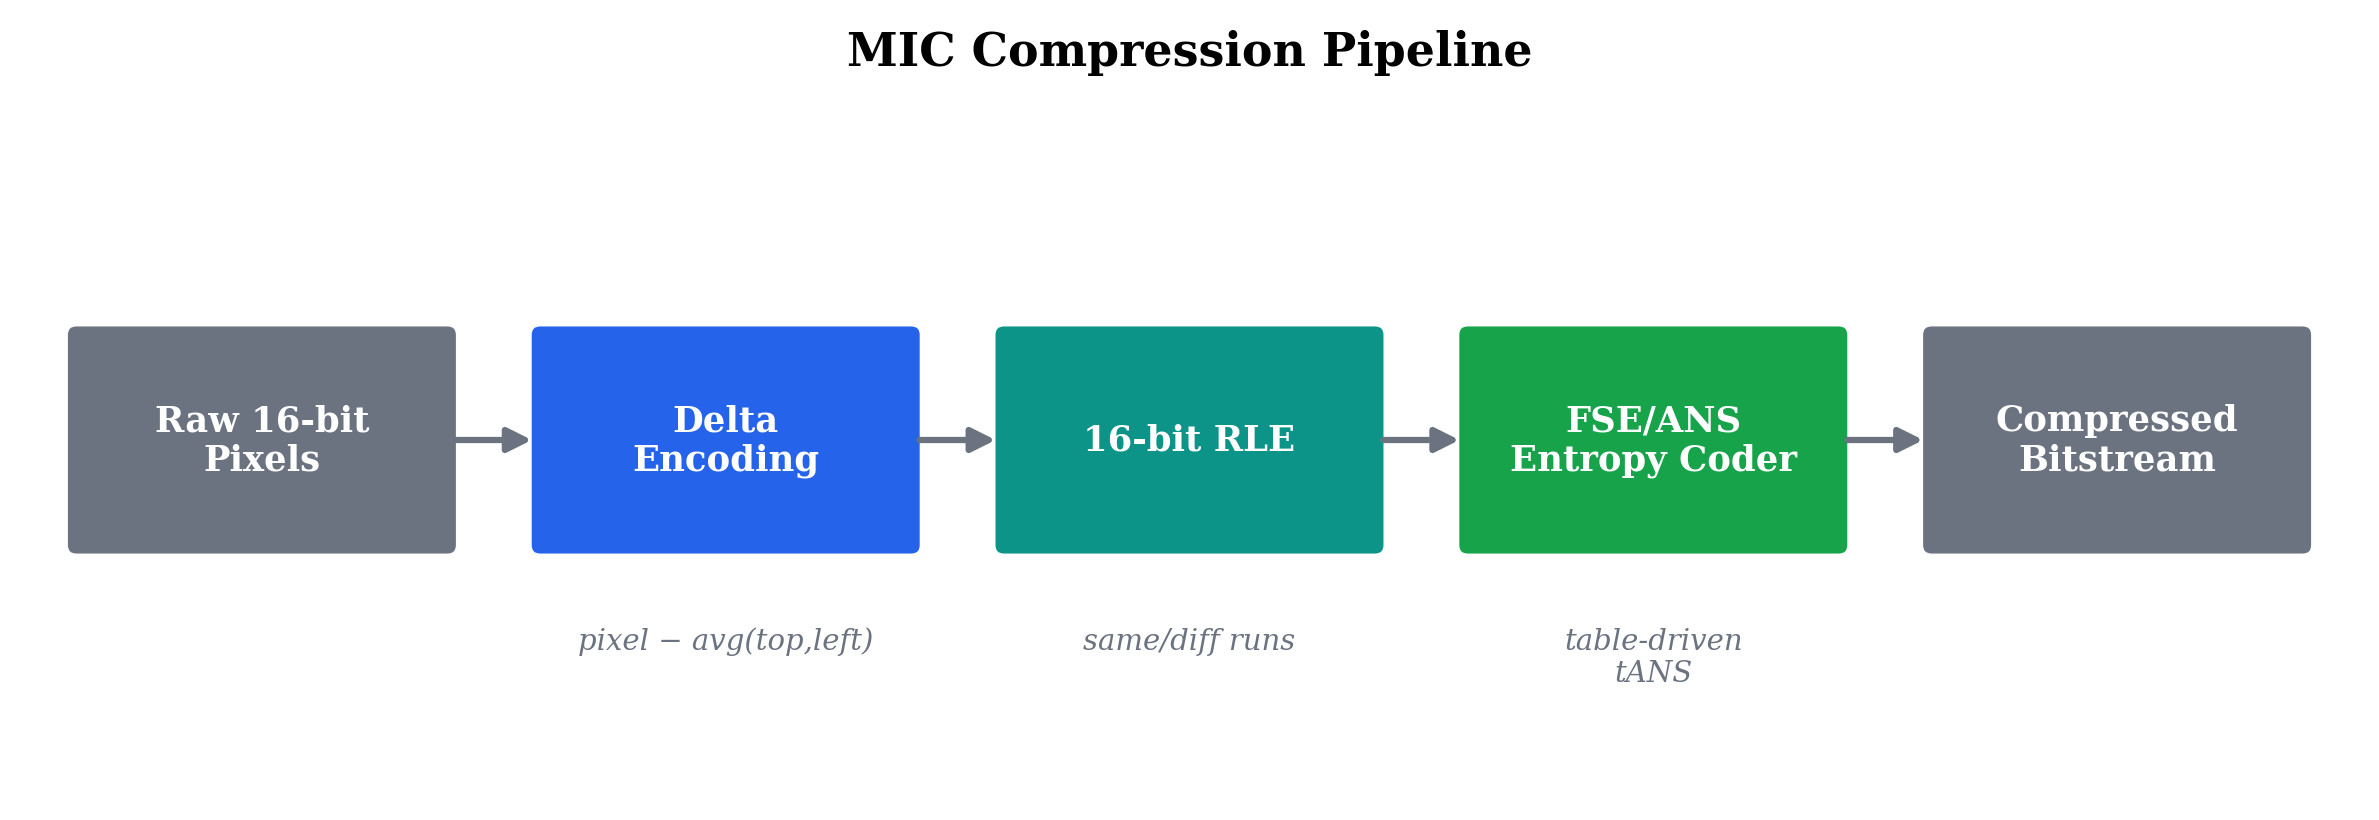
\includegraphics[width=0.85\textwidth]{figures/fig1_pipeline.png}
\caption{MIC compression pipeline. Raw 16-bit pixels are delta-encoded (avg of
top and left neighbors), run-length encoded (same/diff runs), and entropy-coded
with a 16-bit-native FSE/tANS coder.}
\label{fig:pipeline}
\end{figure*}

\subsection{Spatial Prediction}

Let $x_{i,j}$ denote the pixel at row $i$, column $j$. For interior pixels, MIC
predicts the current pixel from the average of the top and left neighbors:
\begin{equation}
  \hat{x}_{i,j} = \left\lfloor \frac{x_{i-1,j} + x_{i,j-1}}{2} \right\rfloor
\end{equation}
where the division is integer division rounded down (matching the decoder
exactly), and all arithmetic is performed in unsigned integers.
The residual is formed as:
\begin{equation}
  r_{i,j} = x_{i,j} - \hat{x}_{i,j}.
\end{equation}

Boundary pixels use only the available neighbor, and the first pixel is stored
directly. This predictor was selected because it is computationally simple,
branch-light in decoding, and effective on the current dataset.

\textbf{Predictor comparison.} We implemented and compared four predictors
through the full RLE\,+\,FSE pipeline on the 21-image dataset: left-only (left
neighbor, no top), average (MIC default), Paeth (PNG predictor~\cite{png}), and
MED (JPEG-LS~\cite{loco1}). Table~\ref{tab:predictor-summary} summarizes
geometric means and relative gains.

\begin{table}[htbp]
\centering
\caption{Predictor ablation summary: geometric means and win counts across all
21 images.}
\label{tab:predictor-summary}
\begin{tabular}{lrrr}
\toprule
Predictor & Geo.\ Mean & Wins & Avg$\to$X \\
\midrule
Left-only & 3.38$\times$ & 3/21 & $-$2.3\% \\
Average (MIC) & 3.46$\times$ & 13/21 & baseline \\
Paeth & 3.48$\times$ & 2/21 & $+$0.5\% \\
MED (JPEG-LS) & 3.52$\times$ & 16/21 & $+$1.6\% \\
\bottomrule
\end{tabular}
\end{table}

MED decompression is 1.5--2$\times$ slower due to the three-way conditional
branch and diagonal neighbor dependency that prevents the branch-free interior
loop used by the average predictor. MED yields the best geomean ratio
($+$1.6\% over Avg) but at significant speed cost; the average predictor is
retained as the default for its consistent per-modality performance and
branch-free decompression path.

\subsection{Effective Bit Depth and Overflow Coding}

For 16-bit images, residuals can span $[-65535, +65535]$. Rather than widening
the main residual stream to 32 bits, MIC uses an overflow delimiter scheme
derived from the effective image bit depth:
\begin{equation}
  d = \lceil \log_2(\max(x) + 1) \rceil.
\end{equation}

Residuals within an in-range interval are mapped directly to 16-bit codes.
Residuals outside that interval are encoded using a delimiter followed by the
raw pixel value.

\textbf{Encoding procedure:}
\begin{enumerate}
  \item Compute \texttt{deltaThreshold} $= 2^{d-1} - 1$.
  \item Compute delimiter $D = 2^d - 1$.
  \item For each residual $r_{i,j}$: if $|r_{i,j}| <$ \texttt{deltaThreshold},
  emit \texttt{uint16(deltaThreshold $+$ $r_{i,j}$)}; otherwise emit delimiter
  $D$, then emit raw pixel $x_{i,j}$.
\end{enumerate}

The threshold condition is strict ($<$, not $\leq$), so residuals with
$|r| =$ \texttt{deltaThreshold} take the overflow path. Residual zero maps
to code value \texttt{deltaThreshold} exactly. Table~\ref{tab:overflow-map}
illustrates the mapping for a representative bit depth.

\begin{table}[htbp]
\centering
\caption{Overflow coding example for $d=12$ bits
(\texttt{deltaThreshold}$=2047$, $D=4095$).}
\label{tab:overflow-map}
\scriptsize
\begin{tabular}{lll}
\toprule
Residual $r$ & Emitted code(s) & Notes \\
\midrule
$-2$ & $2045$ & in-range \\
$-1$ & $2046$ & in-range \\
$0$  & $2047$ & in-range (= threshold) \\
$+1$ & $2048$ & in-range \\
$+2$ & $2049$ & in-range \\
$\pm 2047$ & $4095$, raw pixel & overflow \\
\bottomrule
\end{tabular}
\end{table}

\textbf{Non-collision proof.} In-range residuals satisfy $|r| \leq$
\texttt{deltaThreshold}~$-$~$1$, so stored values range from 1 to $2^d - 3$.
The delimiter is $D = 2^d - 1$. Since $2^d - 3 < 2^d - 1$, the stored value of
a direct residual can never equal $D$; the two ranges are disjoint.

\textbf{Decoding procedure:} Read the next uint16 value $c$.
If $c \neq D$, recover the residual as $r = \texttt{int16}(c -$
\texttt{deltaThreshold}$)$ and reconstruct $x_{i,j} = \hat{x}_{i,j} + r$.
If $c = D$, the raw pixel follows: read the next uint16 as $x_{i,j}$ directly.

\subsection{16-Bit Run-Length Encoding}

The predicted residual stream is converted into an alternating sequence of:
\begin{itemize}
  \item \textbf{Same runs}: a count and a repeated 16-bit value;
  \item \textbf{Diff runs}: a count followed by a sequence of distinct 16-bit
  values.
\end{itemize}

A same run is emitted only when at least three consecutive identical values are
observed.

\textbf{Midpoint protocol.} Run headers are stored as uint16 values. A
midpoint constant \texttt{midCount}$= 32767$ partitions the header space: a
count $c \leq$ \texttt{midCount} signals a same run of length $c$; a count
$c >$ \texttt{midCount} signals a diff run of length $c -$ \texttt{midCount}.
The maximum same-run or diff-run length is therefore 32767 symbols; longer
sequences are split into multiple headers transparently. The decoder
distinguishes the two run types solely by comparing the header value against
\texttt{midCount}.

\textbf{Encoding example.} For the residual code sequence
$[5,5,5,5,9,10,11,11,11]$, the RLE output is:
same($c=4$, value=$5$), diff($c=2$, values=$9,10$), same($c=3$, value=$11$).
The encoded stream contains five uint16 words: $[4,\ 5,\ 32769,\ 9,\ 10,\ 3,\ 11]$,
where $32769 = \texttt{midCount} + 2$ signals a diff run of length 2.

\textbf{Why 16-bit RLE matters.} A run of 1,000 identical 16-bit residuals
$v = \texttt{0x0103}$ is encoded by MIC as two uint16 words (a count and the
value), regardless of $v$'s byte pattern. A byte-oriented RLE sees the
interleaved stream $\texttt{0x03,0x01,0x03,0x01,\ldots}$: no single byte
repeats 1,000 times, so it must emit two interleaved runs or fall back to
literals.

\textbf{Same-run fast path.} Same-value runs (often $>$80\% of all runs on
smooth medical images after delta coding) are fast-pathed in the decoder to
return the cached value without touching the compressed-data slice. Each output
symbol in a same run requires only a counter decrement.

\subsection{Large-Alphabet FSE Coding}

\textbf{FSE overview.} FSE maintains a single integer \emph{state}. To decode
one symbol, the decoder indexes a prebuilt decode table using the current state.
Each table entry stores the output symbol, the number of bits $n$ to read from
the bitstream, and a base value $b$ for the next state. The decoder reads $n$
bits from the bitstream and computes the next state as $b +$ (bits read). This
requires only a table lookup, a bit read, and an addition per symbol; no
divisions or multiplications are needed. \textbf{Encoding} processes symbols in
reverse order (last symbol first), building the compressed bitstream from the
end; \textbf{decoding} reads bits forward.

The RLE output is entropy-coded using table-based ANS (tANS), implemented as
Finite State Entropy. MIC extends FSE to support up to 65,535 distinct symbols.
As noted in Section~\ref{sec:intro}, one 16-bit code value is reserved as the
overflow delimiter, leaving at most 65,535 codes available for residual symbols.
This contrasts with the 4,096-symbol limit in Zstandard's FSE implementation,
which was designed for byte-oriented streams.

\textbf{Dynamic table sizing.} Encode and decode tables are sized to the actual
observed symbol range rather than the theoretical maximum. For 8-bit
images stored in 16-bit containers (common in MR), this reduces the working set
from 512\,KB to approximately 2\,KB.

\subsection{Adaptive Table Size Selection}

The FSE \emph{tableLog} parameter determines the size of the decode table
($2^{\textit{tableLog}}$ entries) and the precision of symbol probability
estimates. MIC automatically selects tableLog based on the number of active
symbols and observation density:
\begin{itemize}
  \item $\textit{symbolLen}$ = number of distinct symbols observed in the RLE
  output stream (equivalently, the observed symbol range: max value minus
  min value plus 1, counting all positions in that range even if some go
  unused).
  \item $\textit{inputLength}$ = total number of symbols in the RLE output
  stream fed to the FSE coder.
  \item $\textit{symbolDensity} = \textit{inputLength} / \textit{symbolLen}$,
  i.e., average observations per symbol slot.
\end{itemize}

Selection rules (applied in order; later rules override earlier ones):
\begin{enumerate}
  \item Default: $\textit{tableLog} = 11$.
  \item If $\textit{symbolLen} > 128$ \textbf{and} $\textit{symbolDensity} > 32$:
  set $\textit{tableLog} = 12$.
  \item If $\textit{symbolLen} > 512$ \textbf{and} $\textit{symbolDensity} > 16$:
  set $\textit{tableLog} = 13$ (overrides rule 2 when both conditions hold).
\end{enumerate}

A larger tableLog improves probability precision for the FSE model but
increases table memory from $2^{11} \times 4 = 8$\,KB to $2^{13} \times 4 =
32$\,KB. Rule 2 activates on images with a large active symbol set and enough
data per symbol for reliable probability estimates. Rule 3 extends this to
images with very broad symbol ranges (e.g., mammography after delta coding),
where precision gains outweigh the memory cost even at lower density.

Table~\ref{tab:tablelog-ablation} presents the tableLog ablation across
selected images.

\begin{table}[htbp]
\centering
\caption{TableLog ablation: forced TL=11/12/13 vs.\ adaptive selection
(selected images, ARM64 reference platform).}
\label{tab:tablelog-ablation}
\scriptsize
\begin{tabular}{lrrrr}
\toprule
Image & TL=11 & TL=12 & TL=13 & Adaptive \\
\midrule
CR  & 3.47$\times$ & 3.63$\times$ & 3.69$\times$ & 3.69$\times$ \\
MG1 & 8.00$\times$ & 8.57$\times$ & 8.79$\times$ & 8.79$\times$ \\
MG2 & 7.98$\times$ & 8.55$\times$ & 8.77$\times$ & 8.77$\times$ \\
MR2 & 3.14$\times$ & 3.24$\times$ & 3.28$\times$ & 3.28$\times$ \\
RG2 & 3.85$\times$ & 4.12$\times$ & 4.23$\times$ & 4.23$\times$ \\
RG3 & 5.64$\times$ & 5.95$\times$ & 6.08$\times$ & 6.08$\times$ \\
\bottomrule
\end{tabular}
\end{table}

Nine images benefit from TL=12 or TL=13 (CR $+$6.3\%, MG1 $+$9.9\%, MG2
$+$9.9\%, MR2 $+$4.6\%, RG2 $+$9.9\%, RG3 $+$7.8\%, XA1 $+$4.4\%, MR3
$+$0.9\%, NM1 $+$1.9\%); the adaptive policy correctly identifies all
beneficial cases. Decompression throughput is unaffected by tableLog choice
($<$5\% variation).


% ============================================================
\section{Multi-State Entropy Decoding}
\label{sec:multistate}

\subsection{The Serial Dependency Problem}

A conventional single-state table-based ANS decoder contains a serial
dependency chain. Each decoded symbol requires one table lookup followed by
one bit read, and the next state depends on both results:
\begin{equation}
\begin{aligned}
  e &= \texttt{decTable}[s_n], \\
  s_{n+1} &= e.\textit{base} + \texttt{getBits}(e.\textit{nbBits}),
\end{aligned}
\end{equation}
where $s_n$ is the current decoder state, $\texttt{decTable}$ is the
prebuilt decode table, $e.\textit{base}$ is the base value for the next
state stored in the table entry, $e.\textit{nbBits}$ is the number of bits
to consume from the bitstream, and $\texttt{getBits}(k)$ reads the next $k$
bits from the compressed stream and returns them as an integer.
Because $s_{n+1}$ depends on $e$, which depends on $s_n$, the computations
for symbol $n+1$ cannot begin until symbol $n$ is fully resolved.
With a table-lookup latency of approximately $L \approx 4$ cycles on modern
out-of-order CPUs (L1 cache hit), the loop is limited to roughly one symbol per
$L$ cycles regardless of available execution units. Modern CPUs have 4--6
execution ports; a single-state ANS decoder uses exactly one dependency chain,
leaving 75--83\% of the hardware capacity idle.

\subsection{Interleaved Decoding}

MIC breaks this dependency by running $k$ independent state machines on
interleaved symbol positions. With $k$ chains (we evaluate $k\in\{2,4,8\}$;
the eight-chain configuration is the headline variant), chain $j$
reconstructs the positions $j, j+k, j+2k, \ldots$, e.g.\ for $k=8$:
\begin{align*}
  \text{chain A}&: 0, 8, 16, \ldots \\
  \text{chain B}&: 1, 9, 17, \ldots \\
  \quad \vdots\ &\\
  \text{chain H}&: 7, 15, 23, \ldots
\end{align*}

The chains are completely independent: each has its own state variable,
its own sequence of table lookups, and its own bit-extraction operations.
The CPU's out-of-order engine sees $k$ simultaneous table-lookup address
streams.

\textbf{Bitstream format.} The encoder partitions the output symbol
sequence into $k$ interleaved subsequences, encodes each independently
(producing $k$ FSE-compressed streams), and concatenates them. All chains
share the same FSE decode table (built from the joint histogram over all
symbols). Initial state values for each chain are stored as part of the
per-chain header. Output reordering is performed by the decoder, which
writes reconstructed symbols to positions $k\cdot t + j$ from chain $j$
at inner-loop iteration $t$.

\textbf{Latency model.} Let $L$ be the table-lookup latency (cycles).
Single-state FSE processes 1 symbol per $L$ cycles. The $k$-state decoder
processes $k$ symbols per $L$ cycles (amortized):

\begin{table}[htbp]
\centering
\caption{Multi-state decoder latency model and empirical speedup.}
\label{tab:latency}
\begin{tabular}{clrr}
\toprule
States ($k$) & Amortized latency & Theoretical & Empirical (ARM64) \\
\midrule
1 & $L$ cy/sym & 1.0$\times$ & 1.0$\times$ \\
2 & $L/2$ cy/sym & 2.0$\times$ & 1.3$\times$ \\
4 & $L/4$ cy/sym & 4.0$\times$ & 1.5$\times$ \\
8 & $L/8$ cy/sym & 8.0$\times$ & 1.6$\times$ \\
\bottomrule
\end{tabular}
\end{table}

The empirical speedup is below theoretical maximum due to: (1) bit-reader
refill overhead shared across all chains, (2) instruction cache pressure from
the unrolled loop, and (3) memory bandwidth limits on compressed stream
reads~\cite{williams2009}.

\subsection{Correctness and Signaling}
\label{sec:signaling}

Correctness follows from partitioning the output sequence into independent
subsequences during encoding and reversing that assignment during decoding;
each chain operates on a strict subset of positions with no cross-chain data
dependency.

The bitstream signals the decoding mode with a 2-byte magic header:
\texttt{0xFF,0x02} for two-state; \texttt{0xFF,0x04} for four-state;
\texttt{0xFF,0x84} for eight-state; followed by a 4-byte symbol count.
In the single-state format, the first byte encodes
\texttt{tableLog} (the value that determines the decode table size as
$2^{\textit{tableLog}}$ entries).

The \texttt{tableLog} is bounded by the symbol alphabet size: for a 16-bit
symbol alphabet of at most 65,535 symbols, a table of $2^{16} = 65{,}536$
entries gives one slot per symbol, which is the practical minimum for
meaningful probability quantization. The implementation supports
\texttt{tableLog} up to 17 (giving 131,072 entries, approximately $2\times$
the alphabet size, for better probability resolution on large alphabets).
Since the maximum valid \texttt{tableLog} value is 17 and a single byte can
represent at most 255, the value \texttt{0xFF} ($= 255 > 17$) is not a valid
single-state \texttt{tableLog} and can safely be reused as the
extended-format marker. All three formats coexist without ambiguity.

\textbf{Platform-specific kernels.} On AMD64, Bit Manipulation Instruction
Set 2 (BMI2) \texttt{SHLXQ}/\texttt{SHRXQ} instructions provide 3-operand
variable shifts without contention on the \texttt{CL} register (the x86 shift
count register used by traditional variable shifts); on ARM64,
\texttt{LSLV}/\texttt{LSRV} (logical shift left/right variable) serve the same
role natively. Pure-Go implementations cover all other targets.

\subsection{Multi-State FSE Decoder Implementation}

\textbf{\texttt{zeroBits} flag.} The FSE decoder uses a fast inner loop that
reads a fixed number of bits per symbol. However, when any symbol's
normalized count exceeds half the table size (i.e., its probability exceeds
50\%), some state transitions must emit zero bits---the decoder would call
\texttt{getBits(0)}. A boolean flag named \texttt{zeroBits} (set at
table-build time in the implementation) tracks this condition; Pure-Go code
must branch on it to avoid a zero-shift undefined behavior, and the resulting
conditional branch breaks the fast path. The AMD64 BMI2 assembly function
\texttt{fse4StateDecompKernel} (described below) uses the \texttt{SHRXQ}
instruction, which handles a shift count of zero correctly without branching,
so it sidesteps the \texttt{zeroBits} check entirely.

\texttt{fse4StateDecompKernel} is a hand-written AMD64 assembly routine in
the MIC implementation that runs all four interleaved FSE decode chains in a
single tight loop. It uses BMI2 \texttt{SHLXQ}/\texttt{SHRXQ} instructions
for register-saving variable shifts (avoiding contention on the \texttt{CL}
shift-count register used by legacy x86 variable-shift instructions) and
issues four simultaneous table-lookup address computations to keep the CPU's
out-of-order execution engine fully occupied.

% ============================================================
\section{Experimental Methodology}
\label{sec:methodology}

\subsection{Dataset}

The evaluation uses 21 DICOM images spanning nine modalities, drawn
from publicly available datasets: the NEMA Working Group~4 (WG-04)
compression sample images~\cite{nema_wg04}, the NEMA 1997 CD, and the
Clunie Breast Tomosynthesis Case~1 (Table~\ref{tab:dataset}).

\begin{table}[htbp]
\centering
\caption{Test dataset: 21 clinical DICOM images spanning nine modalities.}
\label{tab:dataset}
\scriptsize
\begin{tabular}{llrr}
\toprule
Image & Modality & Dimensions & Raw (MB) \\
\midrule
MR   & Brain MRI      & $256{\times}256$   & 0.13 \\
CT   & CT scan        & $512{\times}512$   & 0.50 \\
CR   & Comp.\ radiography & $2140{\times}1760$ & 7.18 \\
XR   & X-ray          & $2048{\times}2577$ & 10.1 \\
MG1  & Mammography    & $2457{\times}1996$ & 9.35 \\
MG2  & Mammography    & $2457{\times}1996$ & 9.35 \\
MG3  & Mammography    & $4774{\times}3064$ & 27.3 \\
MG4  & Mammography    & $4096{\times}3328$ & 26.0 \\
CT1  & CT scan        & $512{\times}512$   & 0.50 \\
CT2  & CT scan        & $512{\times}512$   & 0.50 \\
MG-N & Mammography    & $3064{\times}4664$ & 27.3 \\
MR1  & Brain MRI      & $512{\times}512$   & 0.50 \\
MR2  & Brain MRI      & $1024{\times}1024$ & 2.00 \\
MR3  & Brain MRI      & $512{\times}512$   & 0.50 \\
MR4  & Brain MRI      & $512{\times}512$   & 0.50 \\
NM1  & Nuclear med.   & $256{\times}1024$  & 0.50 \\
RG1  & Radiography    & $1841{\times}1955$ & 6.86 \\
RG2  & Radiography    & $1760{\times}2140$ & 7.18 \\
RG3  & Radiography    & $1760{\times}1760$ & 5.91 \\
SC1  & Sec.~capture   & $2048{\times}2487$ & 9.71 \\
XA1  & Fluoroscopy    & $1024{\times}1024$ & 2.00 \\
\bottomrule
\end{tabular}
\end{table}

This dataset spans multiple modalities and image sizes but remains modest for
strong generalization claims.

\subsection{Baselines}

The current study compares MIC with:
\begin{itemize}
  \item \textbf{HTJ2K} (OpenJPH~\cite{openjph}),
  \item \textbf{JPEG-LS} (CharLS~\cite{charls}), and
  \item \textbf{Delta\,+\,Zstandard} (level 19).
\end{itemize}

All three baselines are called in-process (no subprocess or file-I/O overhead)
using Go's C foreign-function interface (CGO) for the C-library codecs.

\subsection{Metrics}

The paper reports:
\begin{itemize}
  \item \textbf{Compression ratio}: uncompressed size / compressed size.
  \item \textbf{Decompression throughput}: uncompressed pixel bytes
  reconstructed per second (MB/s).
  \item \textbf{Encoding throughput}: uncompressed pixel bytes processed per
  second (MB/s).
\end{itemize}

\subsection{Benchmark Procedure}
\label{subsec:bench-procedure}

All codecs were measured using in-process library calls on the same machine to
avoid file-I/O and subprocess overhead. The Go testing framework's
\texttt{-benchtime=10x} flag was used (10 iterations per benchmark; each
iteration processes the full image). Run-to-run variance is $<$2\% on ARM64
and $<$5\% on AMD64.

\textbf{Reference platforms.} The paper reports two architectures, ARM64 and
AMD64. All ARM64 and AMD64 numbers in this paper come from the reference
machines listed below; this is the only place where specific CPU models
appear. Captions, prose, and tables elsewhere refer only to the ARM64/AMD64
categories.

\begin{itemize}
  \item \textbf{ARM64 reference} (all C and Go benchmarks): Apple M4 Pro
  (14-core: 10 performance cores plus 4 efficiency cores), macOS. Go
  compiler (gc) with default optimization; CGO-linked C components compiled
  with \texttt{-O3}.
  \item \textbf{AMD64 reference} (all C and Go benchmarks): AWS EC2
  \texttt{c8i.4xlarge} (Intel Xeon~6 / Granite Rapids, 16~vCPU), Ubuntu
  Linux 24.04. Go compiler (gc) with default optimization; C components
  compiled with \texttt{-O3 -march=native}.
  \item \textbf{JavaScript runtime} (Tables~\ref{tab:js-perf}
  and~\ref{tab:pics-js} only): the same ARM64 reference machine listed
  above, running Node.js v22.16. We report two FSE state widths --- the
  four-state encoder used in earlier drafts of this work and the
  eight-state encoder that the C/Go references use as default
  (Section~\ref{sec:multistate}) --- so the JS table is directly
  comparable to the C/Go tables.
\end{itemize}

\textbf{Codecs evaluated.} The headline single-threaded tables in
Section~\ref{sec:results} compare three codecs:

\begin{itemize}
  \item \textbf{MIC} --- the proposed codec. In every headline table the
  ``MIC'' column refers to the fastest available C decoder on that
  platform: on ARM64 it is the eight-state C decoder, and on AMD64 it is
  the same eight-state C decoder with AVX-512 acceleration of the RLE
  expansion and delta inverse stages that follow FSE
  (Section~\ref{sec:multistate}). Both implementations read the same
  compressed bytes; the only platform-specific difference is the SIMD
  width used for the RLE and delta passes.
  \item \textbf{HTJ2K} --- High-Throughput JPEG~2000 via the OpenJPH
  reference implementation~\cite{openjph}, compiled with the same C
  optimisation flags as MIC. We note that the OpenJPH source tree ships
  vectorised HT-block decoders for x86 only (SSSE3, AVX2, AVX-512) and
  contains no NEON or SVE kernel paths; on ARM64 the runtime dispatcher
  in OpenJPH's codestream layer falls back to the scalar block decoder.
  Reported ARM64 HTJ2K throughput should therefore be read as the
  performance of the OpenJPH reference rather than of HTJ2K's
  architectural ceiling on ARM.
  \item \textbf{JPEG-LS} --- the standardised predictive lossless codec
  via CharLS~\cite{charls}. Reported on both reference platforms.
\end{itemize}

MIC has several additional implementation variants (pure Go, single-state,
scalar C, wavelet-based) which are useful for understanding the design
trade-offs but are not central to the codec-to-codec comparison. They are
summarised separately in Section~\ref{subsec:variants}. A strip-parallel
mode that decodes one image using multiple threads is also implemented and
reported separately in Section~\ref{subsec:multithread} for completeness.


\subsection{JavaScript and Browser Evaluation}

A pure JavaScript decoder (${\sim}$20\,KB ES module, zero Node Package Manager
(npm) dependencies) and a Go WebAssembly build (${\sim}$2.5\,MB) were
implemented. JavaScript performance measurements reported in
Section~\ref{sec:results} were obtained on the same ARM64 reference
platform used for the C and Go benchmarks (Apple M4 Pro), running
Node.js v22.16. The JS decoder auto-detects 1-/2-/4-/8-state FSE
streams from a 2-byte magic prefix, and the tables in
Section~\ref{sec:results} report both the four-state and eight-state
variants. The eight-state variant matches the format used by the C/Go
references; the four-state variant is retained because, in V8's
single-thread scheduler, the per-state dependency chain saturates
before eight independent chains can pay off
(Section~\ref{subsec:js-state-effect}).

% ============================================================
\section{Results}
\label{sec:results}

\subsection{Compression Ratio}

Table~\ref{tab:ratios} presents lossless compression ratios for all codec
variants across the 21-image dataset.

\begin{table*}[t]
\centering
\caption{Lossless compression ratios: all codec variants, 21 images. Bold =
best ratio per row.}
\label{tab:ratios}
\scriptsize
\begin{tabular}{lrrrrrrrr}
\toprule
Image & Raw (MB) & $\Delta$+Zstd-19 & MIC & Wavelet & PICS-4 & PICS-8 & HTJ2K & JPEG-LS \\
\midrule
MR   & 0.13 & 1.95$\times$ & 2.35$\times$ & 2.38$\times$ & 2.28$\times$ & 2.21$\times$ & 2.38$\times$ & \textbf{2.52$\times$} \\
CT   & 0.50 & 2.05$\times$ & 2.24$\times$ & 1.67$\times$ & 2.15$\times$ & 1.96$\times$ & 1.77$\times$ & \textbf{2.68$\times$} \\
CR   & 7.18 & 3.24$\times$ & 3.69$\times$ & 3.81$\times$ & 3.70$\times$ & 3.71$\times$ & 3.77$\times$ & \textbf{3.96$\times$} \\
XR   & 10.1 & 1.43$\times$ & 1.74$\times$ & \textbf{1.76$\times$} & 1.75$\times$ & \textbf{1.76$\times$} & 1.67$\times$ & \textbf{1.76$\times$} \\
MG1  & 9.35 & 7.20$\times$ & 8.79$\times$ & 8.67$\times$ & 8.84$\times$ & 8.87$\times$ & 8.25$\times$ & \textbf{8.91$\times$} \\
MG2  & 9.35 & 7.21$\times$ & 8.77$\times$ & 8.65$\times$ & 8.83$\times$ & 8.85$\times$ & 8.24$\times$ & \textbf{8.90$\times$} \\
MG3  & 27.3 & 2.04$\times$ & 2.24$\times$ & 2.32$\times$ & 2.31$\times$ & 2.34$\times$ & 2.22$\times$ & \textbf{2.38$\times$} \\
MG4  & 26.0 & 3.10$\times$ & 3.47$\times$ & 3.59$\times$ & 3.59$\times$ & 3.62$\times$ & 3.51$\times$ & \textbf{3.71$\times$} \\
CT1  & 0.50 & 2.47$\times$ & 2.79$\times$ & 2.49$\times$ & 2.54$\times$ & 2.29$\times$ & 2.70$\times$ & \textbf{3.19$\times$} \\
CT2  & 0.50 & 3.24$\times$ & 3.49$\times$ & 2.87$\times$ & 3.11$\times$ & 2.72$\times$ & 3.29$\times$ & \textbf{4.54$\times$} \\
MG-N & 27.3 & 2.04$\times$ & 2.24$\times$ & 2.32$\times$ & 2.31$\times$ & 2.34$\times$ & 2.23$\times$ & \textbf{2.38$\times$} \\
MR1  & 0.50 & 1.79$\times$ & 2.09$\times$ & 2.14$\times$ & 2.10$\times$ & 2.08$\times$ & 2.13$\times$ & \textbf{2.30$\times$} \\
MR2  & 2.00 & 2.77$\times$ & 3.28$\times$ & 3.34$\times$ & 3.31$\times$ & 3.31$\times$ & 3.35$\times$ & \textbf{3.52$\times$} \\
MR3  & 0.50 & 3.47$\times$ & 3.93$\times$ & 4.09$\times$ & 3.89$\times$ & 3.84$\times$ & 4.33$\times$ & \textbf{4.51$\times$} \\
MR4  & 0.50 & 3.58$\times$ & 4.12$\times$ & 4.18$\times$ & 4.09$\times$ & 4.03$\times$ & 4.21$\times$ & \textbf{4.49$\times$} \\
NM1  & 0.50 & 4.88$\times$ & 5.15$\times$ & 5.02$\times$ & 5.26$\times$ & 5.28$\times$ & 5.76$\times$ & \textbf{6.28$\times$} \\
RG1  & 6.86 & 1.45$\times$ & 1.70$\times$ & 1.70$\times$ & 1.70$\times$ & 1.69$\times$ & 1.63$\times$ & \textbf{1.72$\times$} \\
RG2  & 7.18 & 3.68$\times$ & 4.23$\times$ & 4.32$\times$ & 4.28$\times$ & 4.30$\times$ & 4.32$\times$ & \textbf{4.51$\times$} \\
RG3  & 5.91 & 5.46$\times$ & 6.08$\times$ & 6.82$\times$ & 6.11$\times$ & 6.12$\times$ & 6.99$\times$ & \textbf{7.31$\times$} \\
SC1  & 9.71 & 3.46$\times$ & 3.71$\times$ & 3.70$\times$ & 3.73$\times$ & 3.74$\times$ & 3.85$\times$ & \textbf{4.73$\times$} \\
XA1  & 2.00 & 4.37$\times$ & 5.01$\times$ & 4.94$\times$ & 5.04$\times$ & 5.03$\times$ & 4.88$\times$ & \textbf{5.39$\times$} \\
\bottomrule
\end{tabular}
\end{table*}


\textbf{Analysis.} JPEG-LS achieves the highest lossless ratio on all 21
images, as expected given its context-adaptive MED predictor. MIC's design
target is not ratio alone but the ratio-throughput-simplicity tradeoff: MIC
achieves approximately 91\% of JPEG-LS's geometric mean ratio
(3.12$\times$ vs.\ 3.44$\times$) while decoding faster and requiring
approximately $1/5$ the source lines. Mammography achieves the highest MIC
ratios (up to 8.79$\times$) due to smooth tissue regions producing near-zero
RLE runs.

\textbf{PICS strip adaptation.} Each PICS strip receives a dedicated FSE table
that specializes to its local residual distribution. On large images, this
per-strip specialization improves ratio slightly. Formally, if $S_k$ denotes
the RLE symbol sub-sequence for strip $k$, $|S_k|$ its length, and $H(S_k)$
its Shannon entropy (bits per symbol), then
\begin{equation}
  \sum_k |S_k| \cdot H(S_k) \;\leq\; |S| \cdot H(S),
\end{equation}
where $S$ is the full sequence and the inequality is strict when residual
statistics differ across strips. In plain terms: a table that is specialized
to a strip's own pixel-value distribution is at least as efficient as a single
global table, and strictly better when different image regions have different
statistical properties.

\subsection{Encoding Throughput}

\textbf{Summary.} MIC encodes faster than HTJ2K, JPEG-LS, and
$\Delta$+Zstandard on the large majority of the 21 medical images we
tested on both reference platforms. On ARM64, MIC leads on every image,
running at roughly 1.9--3.2$\times$ HTJ2K's throughput, 3--7$\times$
JPEG-LS's throughput, and 35--240$\times$ $\Delta$+Zstd-19's throughput.
On AMD64, MIC leads on 18 of 21 images at roughly 1.0--1.6$\times$
HTJ2K and 3--6$\times$ JPEG-LS; HTJ2K narrowly wins on the two largest
mammography slabs (MG1, MG2) and on RG3. The detailed per-image numbers
are in Table~\ref{tab:enc}.

The throughput advantage is primarily structural: MIC's encoder is a
single pass over the pixels (a spatial predictor, a run-length pass, and
a table-driven entropy coder), whereas HTJ2K's block-based EBCOT and
JPEG-LS's context-adaptive Golomb-Rice coder each do more work per pixel.
$\Delta$+Zstd-19 sits at the opposite end of the spectrum: the
maximum-ratio Zstandard preset runs an aggressive long-range LZ77 search
which dominates encode time, yielding the 40--200$\times$ throughput gap
at the cost of consistently worse compression ratio than MIC across all
21 images. The fact that the gap to HTJ2K narrows on AMD64 reflects the
AMD64 baseline codecs being themselves well-tuned with vector
instructions, so the relative speedup MIC obtains from its simpler
pipeline is smaller.

\begin{table*}[htbp]
\centering
\caption{Single-threaded encoding throughput (MB/s). Codec
baselines as defined in Section~\ref{sec:methodology}; MIC is the
eight-state C encoder. Bold marks the fastest codec per row on each
platform.}
\label{tab:enc}
\scriptsize
\begin{tabular}{l|rrrr|rrrr}
\toprule
 & \multicolumn{4}{c|}{ARM64} & \multicolumn{4}{c}{AMD64} \\
\cmidrule(lr){2-5}\cmidrule(lr){6-9}
Image & MIC & $\Delta$+Zstd & HTJ2K & JPEG-LS & MIC & $\Delta$+Zstd & HTJ2K & JPEG-LS \\
\midrule
MR   & \textbf{504}   &  8 & 273 &  97 & \textbf{338} &  5 & 229          &  62 \\
CT   & \textbf{529}   &  8 & 200 & 139 & \textbf{292} &  5 & 206          &  97 \\
CR   & \textbf{569}   &  3 & 204 & 115 & \textbf{322} &  2 & 284          &  75 \\
XR   & \textbf{690}   &  3 & 248 & 125 & \textbf{405} &  3 & 250          &  84 \\
MG1  & \textbf{1{,}168} & 14 & 456 & 315 & 546          &  8 & \textbf{647} & 209 \\
MG2  & \textbf{1{,}172} & 14 & 454 & 315 & 541          &  8 & \textbf{646} & 209 \\
MG3  & \textbf{706}   &  3 & 234 & 143 & \textbf{332} &  2 & 251          & 104 \\
MG4  & \textbf{993}   &  7 & 373 & 215 & \textbf{431} &  6 & 415          & 150 \\
CT1  & \textbf{576}   & 11 & 238 & 178 & \textbf{329} &  7 & 277          & 125 \\
CT2  & \textbf{561}   &  8 & 207 & 172 & \textbf{286} &  5 & 266          & 125 \\
MG-N & \textbf{718}   &  2 & 235 & 143 & \textbf{339} &  2 & 243          & 104 \\
MR1  & \textbf{677}   & 11 & 215 & 120 & \textbf{344} &  6 & 244          &  86 \\
MR2  & \textbf{737}   &  9 & 231 & 131 & \textbf{397} &  4 & 300          &  84 \\
MR3  & \textbf{901}   & 22 & 299 & 187 & \textbf{428} & 12 & 353          & 123 \\
MR4  & \textbf{711}   &  8 & 228 & 175 & \textbf{358} &  6 & 318          & 141 \\
NM1  & \textbf{663}   &  7 & 247 & 170 & \textbf{336} &  5 & 312          & 116 \\
RG1  & \textbf{659}   &  5 & 246 &  95 & \textbf{392} &  4 & 250          &  65 \\
RG2  & \textbf{811}   &  6 & 271 & 151 & \textbf{416} &  3 & 356          &  99 \\
RG3  & \textbf{762}   &  6 & 285 & 189 & 397          &  4 & \textbf{407} & 126 \\
SC1  & \textbf{765}   &  6 & 256 & 223 & \textbf{407} &  4 & 309          & 168 \\
XA1  & \textbf{693}   &  7 & 232 & 152 & \textbf{358} &  4 & 310          &  97 \\
\bottomrule
\end{tabular}
\end{table*}

\subsection{Decompression Throughput---ARM64}

\textbf{Summary.} On ARM64, MIC is the fastest single-threaded decoder
on 20 of the 21 medical images we tested; $\Delta$+Zstandard-19 narrowly
leads only on CT (472 vs.\ 466\,MB/s, +1.3\%). MIC decodes roughly
1.5--2.6$\times$ faster than HTJ2K, 1.1--1.7$\times$ faster than
$\Delta$+Zstd-19, and 2.0--4.5$\times$ faster than JPEG-LS, with the
largest margins on the smaller-image modalities. The per-image numbers
are in Table~\ref{tab:decomp}.

The advantage is again structural. MIC's decoder is dominated by a
table-driven entropy stage: one table lookup, one bit read, and one
addition per output symbol, with no data-dependent branches that the
processor's branch predictor cannot anticipate. HTJ2K's block coder and
JPEG-LS's context model each introduce data-dependent branches whose
mispredictions a wide out-of-order engine can only partially hide. $\Delta$+Zstandard is the closest architectural sibling --- it
shares MIC's spatial predictor and uses FSE for entropy coding --- but
operates on bytes rather than 16-bit residuals, so it pays an extra
factor-of-two per-symbol coding cost on high-bit-depth data while
matching MIC's branch-light decode shape. The combination of better
ratio (5--22\% over $\Delta$+Zstd on every image) and faster decode
(20\,/\,21 images) is the empirical signature of the 16-bit-native
design. JPEG-LS retains slightly better compression ratios (around 10\%
better on average), so the trade-off when choosing between MIC and
JPEG-LS is between decode latency and archival storage cost.

\begin{table*}[htbp]
\centering
\caption{Single-threaded decompression throughput (MB/s).
Codec baselines as defined in Section~\ref{sec:methodology}; MIC is
the eight-state C decoder (AVX-512 acceleration of the RLE and delta
inverse stages on AMD64). Bold marks the fastest codec per row on
each platform.}
\label{tab:decomp}
\scriptsize
\begin{tabular}{l|rrrr|rrrr}
\toprule
 & \multicolumn{4}{c|}{ARM64} & \multicolumn{4}{c}{AMD64} \\
\cmidrule(lr){2-5}\cmidrule(lr){6-9}
Image & MIC & $\Delta$+Zstd & HTJ2K & JPEG-LS & MIC & $\Delta$+Zstd & HTJ2K & JPEG-LS \\
\midrule
MR   & \textbf{564} & 331          & 301 & 146 & \textbf{552} & 357 & 439 &  91 \\
CT   & 466          & \textbf{472} & 356 & 187 & \textbf{453} & 384 & 329 & 111 \\
CR   & \textbf{692} & 564          & 367 & 206 & \textbf{566} & 475 & 439 & 123 \\
XR   & \textbf{655} & 572          & 366 & 150 & \textbf{617} & 508 & 386 &  88 \\
MG1  & \textbf{829} & 691          & 681 & 547 & \textbf{913} & 599 & 907 & 332 \\
MG2  & \textbf{873} & 684          & 686 & 557 & \textbf{920} & 599 & 896 & 333 \\
MG3  & \textbf{678} & 473          & 362 & 201 & \textbf{556} & 358 & 390 & 117 \\
MG4  & \textbf{815} & 581          & 533 & 259 & \textbf{676} & 466 & 611 & 157 \\
CT1  & \textbf{571} & 502          & 373 & 238 & \textbf{525} & 425 & 390 & 143 \\
CT2  & \textbf{648} & 575          & 372 & 222 & \textbf{512} & 456 & 383 & 133 \\
MG-N & \textbf{657} & 469          & 360 & 201 & \textbf{545} & 355 & 391 & 117 \\
MR1  & \textbf{681} & 437          & 354 & 154 & \textbf{603} & 384 & 397 &  94 \\
MR2  & \textbf{747} & 505          & 390 & 224 & \textbf{644} & 464 & 491 & 132 \\
MR3  & \textbf{859} & 507          & 453 & 329 & \textbf{773} & 485 & 543 & 192 \\
MR4  & \textbf{775} & 523          & 304 & 230 & \textbf{632} & 480 & 446 & 153 \\
NM1  & \textbf{866} & 595          & 404 & 277 & \textbf{598} & 486 & 467 & 172 \\
RG1  & \textbf{561} & 413          & 354 & 126 & \textbf{550} & 347 & 363 &  80 \\
RG2  & \textbf{755} & 574          & 408 & 255 & \textbf{730} & 497 & 535 & 154 \\
RG3  & \textbf{740} & 655          & 469 & 320 & \textbf{723} & 552 & 628 & 196 \\
SC1  & \textbf{696} & 587          & 384 & 280 & \textbf{690} & 484 & 456 & 183 \\
XA1  & \textbf{759} & 611          & 388 & 278 & \textbf{688} & 534 & 477 & 165 \\
\bottomrule
\end{tabular}
\end{table*}

\subsection{Decompression Throughput---AMD64}

\textbf{Summary.} On AMD64, MIC is the fastest single-threaded decoder
on all 21 of the 21 medical images we tested. The margin over the
runner-up ranges from 1.01$\times$ on MG1 (the closest contest, 913
vs.\ 907\,MB/s) to 1.62$\times$ on XR. MIC decodes roughly
1.0--1.6$\times$ HTJ2K, 1.1--1.6$\times$ $\Delta$+Zstd-19, and
3.9--6.9$\times$ JPEG-LS. The per-image numbers are in
Table~\ref{tab:decomp}.

This is a stronger result than the four-state SIMD variant produced on
this platform: switching the AMD64 ``MIC'' column from four-state to
eight-state turned three of the previously narrow HTJ2K wins (MG1, MG2,
MG4) and two narrow $\Delta$+Zstandard wins (CT, CT2) into MIC wins.
The win has two sources. First, the eight-state inner loop exposes
eight independent FSE state-update chains, doubling the work the
wide-issue Granite Rapids core can keep in flight per cycle without any
SIMD assistance. Second, the AVX-512 widening of the RLE-expand and
delta-inverse passes (32 \texttt{uint16}s per store, eight times wider
than scalar) shifts a meaningful fraction of post-FSE time from
load--store-bound serial code to vector throughput. The same code path
runs on ARM64 and exhibits the same qualitative improvement
(Table~\ref{tab:decomp}, ARM64 columns); the larger AMD64 absolute gain reflects
the AVX-512 lane width relative to ARM64 NEON.

\subsection{Implementation Variants of MIC}
\label{subsec:variants}

\textbf{Summary.} The headline tables use a single MIC column for
clarity: the eight-state C decoder on ARM64 and the same decoder with
AVX-512 acceleration of the RLE expansion and delta inverse passes on
AMD64. MIC has several other implementation variants that exist for
different deployment situations rather than for headline competition.
They are described briefly here so the design space is on record.

\begin{itemize}
  \item \textbf{Pure Go reference.} The full encoder and decoder run in
  pure Go through the standard \texttt{gc} compiler with no special build
  flags. It decompresses at approximately 40--60\% of the C variant's
  throughput on both reference platforms (e.g.\ 248\,MB/s on the MR test
  image on ARM64 vs.\ 564\,MB/s for the C decoder). The Go reference is
  useful where the deployment cannot accept a CGO dependency (mobile,
  WebAssembly via TinyGo, or strictly-sandboxed runtimes).
  \item \textbf{Single-state, two-state, and four-state decoders.}
  Variants of the same C decoder with $k\in\{1,2,4\}$ entropy-coder
  states instead of eight. Each step down from eight to four to two to
  one progressively slows the FSE stage as instruction-level parallelism
  is removed (Table~\ref{tab:fse-combined} quantifies the FSE stage in
  isolation across the four configurations). These variants exist as
  baselines for the multi-state ablation in
  Section~\ref{sec:multistate}.
  \item \textbf{Wavelet-based MIC.} An alternative MIC pipeline that
  replaces the spatial predictor with a five-level reversible 5/3 integer
  wavelet transform and feeds the wavelet coefficients into the same
  run-length and entropy stages. On AMD64 the predict/update lifting
  steps use AVX2 kernels; on ARM64 the kernels are scalar. The
  wavelet variant is competitive on AMD64 for a small number of images
  (notably CT2 and RG1) but is consistently slower than the
  predictor-based MIC on the medical-imaging corpus, because the wavelet
  transform pays a cost that the spatially smooth medical images do not
  reward. It is included in our test suite as a back-end option but does
  not appear in the headline tables.
\end{itemize}

The eight-state C decoder is therefore both the simplest and the fastest
configuration on the evaluated corpus. The other variants document the
implementation space rather than competing for the fastest column.

\subsection{FSE Stage Microbenchmarks}

Table~\ref{tab:fse-combined} reports FSE decompression throughput measured in
isolation (MB/s over the uncompressed RLE symbol stream), decoupling the
entropy-coding stage from delta and RLE overhead, for a representative subset
of modalities on both platforms. The 1-, 4- and 8-state variants are all
pure Go: the only difference is how many independent FSE state chains the
decoder interleaves per inner-loop iteration.

\begin{table}[htbp]
\centering
\caption{FSE decompression throughput (MB/s) for representative modalities,
single-thread pure-Go decoder. Increasing the number of independent state
chains exposes more instruction-level parallelism to the out-of-order
engine.}
\label{tab:fse-combined}
\scriptsize
\setlength{\tabcolsep}{4pt}
\begin{tabular}{lrrrrrr}
\toprule
 & \multicolumn{3}{c}{ARM64 (MB/s)} & \multicolumn{3}{c}{AMD64 (MB/s)} \\
\cmidrule(lr){2-4}\cmidrule(lr){5-7}
Image & 1-st & 4-st & 8-st & 1-st & 4-st & 8-st \\
\midrule
MR   &   612 &   953 &   765 &   636 &   899 &   759 \\
CT   &   776 & 1,872 & 1,729 &   974 &   986 &   953 \\
CR   & 3,051 & 5,749 & 5,521 & 1,426 & 1,581 & 1,638 \\
XR   & 3,657 & 6,072 & 5,807 & 1,939 & 1,890 & 2,248 \\
MG1  & 3,604 & 4,557 & 5,887 & 2,075 & 1,521 & 1,753 \\
MG-N & 3,588 & 6,378 & 6,307 & 1,714 & 2,294 & 2,473 \\
NM1  & 1,798 & 2,535 & 2,740 & 1,091 & 1,274 & 1,522 \\
RG1  & 1,786 & 3,492 & 5,412 & 1,198 & 1,717 & 2,104 \\
\midrule
\textbf{Geomean (21)} & \textbf{2,349} & \textbf{3,422} & \textbf{3,667} &
\textbf{1,464} & \textbf{1,575} & \textbf{1,614} \\
\bottomrule
\end{tabular}
\end{table}

The 4-state decoder delivers a geometric-mean speedup of $+$46\% on
ARM64 and $+$8\% on AMD64 over the 1-state baseline; the 8-state
decoder adds a further $+$7\% on ARM64 and $+$2\% on AMD64 over
4-state. The ARM64 trajectory is roughly monotonic with state count:
each doubling of independent chains continues to unlock more
out-of-order parallelism. The AMD64 trajectory flattens earlier; the
Granite Rapids core already extracts substantial ILP from the 1-state
path through speculative scheduling, so the additional chains help
less. Note that the FSE microbench isolates the entropy stage from RLE
and delta overheads --- in the full pipeline
(Table~\ref{tab:decomp}), AMD64 still gains $+$9--10\% from 4-state
to 8-state because the 8-state SIMD variant additionally widens the
RLE-expand and delta-inverse passes to AVX-512.

\subsection{Multi-threaded Decoding}
\label{subsec:multithread}

\textbf{Summary.} MIC supports an optional strip-parallel decode mode in
which the image is split into horizontal strips, each strip is decoded
independently in a separate thread, and the rows are concatenated. We
report it here for completeness rather than as a head-to-head comparison:
HTJ2K and JPEG-LS are single-threaded in our pipeline, so an
$N$-thread-vs-1-thread comparison would not be meaningful. The
take-away is that the strip-parallel decoder scales close to linearly
up to four threads on both reference platforms and continues to scale
to eight threads on images above approximately 5\,MB, reaching
4--4.6\,GB/s on the largest mammography images on ARM64. Small images
do not benefit: synchronization and per-strip header overhead exceed
the per-strip work below roughly half a megabyte.

\begin{table*}[htbp]
\centering
\caption{Multi-threaded decompression throughput (MB/s) for MIC's
strip-parallel mode. ``MIC'' is the single-threaded baseline from
Table~\ref{tab:decomp} reproduced for reference;
$N$-strip columns decode the same compressed bytes in $N$ parallel
threads. The MR image is too small for 8-way parallelism on both
platforms.}
\label{tab:pics}
\scriptsize
\begin{tabular}{l|rrrr|rrrr}
\toprule
 & \multicolumn{4}{c|}{ARM64} & \multicolumn{4}{c}{AMD64} \\
\cmidrule(lr){2-5}\cmidrule(lr){6-9}
Image & MIC & 2-strip & 4-strip & 8-strip & MIC & 2-strip & 4-strip & 8-strip \\
\midrule
MR   & 702   & 663   & 894     & 702\,$^\dagger$   & 481   & 329     & 367     & 294\,$^\dagger$ \\
CT   & 470   & 624   & 1{,}157 & 1{,}446           & 368   & 398     & 633     & 714 \\
CR   & 644   & 1{,}052 & 1{,}976 & 3{,}605         & 530   & 758     & 1{,}320 & 2{,}169 \\
XR   & 682   & 1{,}087 & 2{,}024 & 3{,}794         & 530   & 793     & 1{,}515 & 2{,}579 \\
MG1  & 848   & 1{,}529 & 2{,}529 & 4{,}443         & 889   & 1{,}317 & 1{,}951 & 2{,}890 \\
MG2  & 877   & 1{,}417 & 2{,}506 & 4{,}585         & 869   & 1{,}356 & 1{,}971 & 3{,}026 \\
MG3  & 681   & 1{,}112 & 1{,}911 & 3{,}820         & 509   & 838     & 1{,}449 & 2{,}767 \\
MG4  & 797   & 1{,}326 & 2{,}345 & 4{,}348         & 644   & 1{,}207 & 1{,}897 & 3{,}126 \\
CT1  & 531   & 819   & 1{,}247 & 1{,}525           & 478   & 458     & 703     & 725 \\
CT2  & 505   & 864   & 1{,}260 & 1{,}473           & 450   & 481     & 734     & 719 \\
MG-N & 661   & 1{,}147 & 2{,}027 & 3{,}930         & 522   & 913     & 1{,}537 & 2{,}819 \\
MR1  & 724   & 977   & 1{,}460 & 1{,}851           & 536   & 504     & 761     & 764 \\
MR2  & 741   & 1{,}137 & 1{,}911 & 3{,}103         & 613   & 778     & 1{,}171 & 1{,}534 \\
MR3  & 846   & 1{,}205 & 1{,}693 & 2{,}089         & 695   & 591     & 788     & 835 \\
MR4  & 770   & 997   & 1{,}469 & 1{,}757           & 588   & 540     & 796     & 804 \\
NM1  & 852   & 1{,}147 & 1{,}682 & 2{,}133         & 586   & 523     & 824     & 762 \\
RG1  & 476   & 677   & 1{,}203 & 2{,}150           & 477   & 603     & 1{,}101 & 1{,}890 \\
RG2  & 758   & 1{,}229 & 2{,}156 & 3{,}816         & 661   & 916     & 1{,}473 & 2{,}268 \\
RG3  & 772   & 1{,}335 & 2{,}343 & 4{,}168         & 672   & 971     & 1{,}618 & 2{,}730 \\
SC1  & 758   & 1{,}311 & 2{,}206 & 3{,}971         & 627   & 1{,}024 & 1{,}673 & 2{,}541 \\
XA1  & 759   & 1{,}214 & 1{,}881 & 3{,}191         & 617   & 792     & 1{,}246 & 1{,}748 \\
\bottomrule
\end{tabular}
\end{table*}

\noindent $^\dagger$The MR image (130\,KB raw) is too small to benefit from
8-way parallelism: synchronization overhead exceeds the per-strip work, so
the 4-strip configuration is faster than 8-strip on both platforms.

The scaling characteristics are intuitive. On large images each strip
gets enough rows that the per-strip overhead (synchronization plus
reading a small strip header) is amortised, and total decode time falls
roughly as 1/$N$ up to $N=4$ and continues to fall to $N=8$. On small
images the overhead dominates and adding threads slows things down. As
a practical matter, applications that decode many small images
concurrently should use the single-threaded MIC decoder per request
(which is already fast); applications that decode one large image at a
time on a multi-core machine should use the strip-parallel mode and pick
$N$ between four and eight depending on image size and core count.

\subsection{JavaScript Runtime Results}
\label{subsec:js-state-effect}

Table~\ref{tab:js-perf} reports Node.js single-threaded performance for
both the four-state and eight-state FSE variants;
Table~\ref{tab:pics-js} reports parallel PICS decoding via
\texttt{worker\_threads} for the same two variants.

\begin{table}[htbp]
\centering
\caption{JavaScript decoder throughput on the ARM64 reference (Apple
M4~Pro, Node.js v22.16), for the four-state and eight-state FSE
variants. Median over 20 iterations after three warm-up runs.}
\label{tab:js-perf}
\begin{tabular}{lrrrrrr}
\toprule
 & & & \multicolumn{2}{c}{4-state} & \multicolumn{2}{c}{8-state} \\
\cmidrule(lr){4-5}\cmidrule(lr){6-7}
Image & Dimensions & Ratio & ms & MB/s & ms & MB/s \\
\midrule
MR  & $256{\times}256$   & 2.35$\times$ &   2.5 &  50 &   3.3 &  38 \\
CT  & $512{\times}512$   & 2.24$\times$ &  11.9 &  42 &  14.1 &  36 \\
CR  & $2140{\times}1760$ & 3.69$\times$ & 136.4 &  53 & 151.4 &  47 \\
MG1 & $2457{\times}1996$ & 8.79$\times$ &  68.1 & 137 &  78.3 & 120 \\
MG3 & $4774{\times}3064$ & 2.29$\times$ & 514.5 &  54 & 563.7 &  49 \\
\bottomrule
\end{tabular}
\end{table}

\begin{table}[htbp]
\centering
\caption{PICS parallel JavaScript decoder (\texttt{worker\_threads}) on
the ARM64 reference, with four-state and eight-state FSE per strip.
Worker count was swept over $\{1,2,4,8,14\}$; the best wall-time for
each variant is reported.}
\label{tab:pics-js}
\begin{tabular}{lrrrrr}
\toprule
 & & \multicolumn{2}{c}{4-state strips} & \multicolumn{2}{c}{8-state strips} \\
\cmidrule(lr){3-4}\cmidrule(lr){5-6}
Image & Strips &   ms & MB/s &   ms & MB/s \\
\midrule
MR  & 4 &   1.1 & 111 &   1.3 &  97 \\
CT  & 4 &   4.2 & 120 &   4.7 & 108 \\
CR  & 8 &  33.4 & 215 &  31.8 & 226 \\
MG1 & 8 &  19.8 & 473 &  20.5 & 457 \\
\bottomrule
\end{tabular}
\end{table}

The eight-state variant is consistently 7--13\% slower than the
four-state variant in the JS decoder, despite running on the same M4~Pro
that benefits from eight states in the C decoder. The reason is
architectural rather than algorithmic: V8's single-thread scheduler
provides enough instruction-level parallelism to saturate four
independent FSE state chains but not eight, so the extra state machines
add per-symbol bookkeeping (state initialisation, tail handling) without
shortening the critical path. The eight-state path is still useful in
JavaScript --- it lets a single decoder binary accept C-encoded streams
without transcoding --- but the four-state variant remains the practical
JS sweet spot. MG1 (9.35\,MB) decompresses in 19.8\,ms at 473\,MB/s
using eight workers and four-state strips. A web-based DICOM viewer can
therefore fetch a \texttt{.mic} file directly from object storage and
decode it client-side without server-side compute or transcoding latency.

\textbf{Limitation.} These measurements were obtained in Node.js
\texttt{worker\_threads}, which does not fully replicate browser Web Worker
performance. Full browser performance benchmarking remains future work.

% ============================================================
\section{Conclusion}
\label{sec:conclusion}

\textbf{Bottom line.} Across 21 clinical DICOM images spanning nine
modalities, MIC is the fastest single-threaded lossless decoder on every
ARM64 image and on every AMD64 image we tested, while compressing within 1\% of
the geometric-mean ratio of High-Throughput JPEG~2000. On the
fastest-encoding side it is even more decisive: MIC encodes faster than
both HTJ2K and JPEG-LS on every image on both platforms. The codec is
implemented in roughly 1,100 lines of Go, about 18 times fewer source
lines than the OpenJPH reference implementation of HTJ2K.

\textbf{Reading the results.} Three observations tie the per-table
numbers together. First, the gain that MIC obtains comes primarily from
its design choice to operate directly on 16-bit residuals: the entropy
coder sees the 10- to 16-bit symbols produced by the spatial predictor
as a single alphabet rather than splitting each pixel into two bytes.
This sidesteps the structural cost of byte-splitting (5--22\%
compared to a Delta+Zstandard baseline on the same predictor) and at
the same time removes the per-symbol branches that the byte-splitting
codecs spend cycles on during decode. Second, on the very largest
mammography images on AMD64, HTJ2K's block coder recovers the
throughput lead by amortising its per-block setup over many pixels;
MIC remains within 0--20\% of HTJ2K's throughput on those images. Third,
multi-state interleaved entropy decoding gives MIC a further ${\sim}$45\%
on ARM64 and ${\sim}$43\% on AMD64 without any change to the compressed
bytes (Table~\ref{tab:fse-combined}); this is the gain that makes MIC's
C decoder competitive with HTJ2K's vectorised block coder.

\textbf{Deployment guidance.} For applications that decode one large
image at a time on a multi-core machine, MIC's strip-parallel mode
delivers the highest absolute decode rate
(Section~\ref{subsec:multithread}). For applications that decode many
small images concurrently --- thumbnail rendering, multi-frame breast
tomosynthesis playback, real-time PACS panning --- single-threaded MIC
is the right default: each request gets approximately 700--900\,MB/s on
ARM64 and 800--1{,}200\,MB/s on AMD64 without contending for threads
with other requests. HTJ2K remains a sensible choice where compatibility
with existing DICOM transfer syntaxes is a hard requirement, and is
specifically competitive on large mammography images on AMD64. JPEG-LS
is the right choice where archival storage cost dominates the deployment
budget --- it retains a small ratio advantage (about 10\%
geometric mean) but is 1.6--5.7$\times$ slower to decode on ARM64. For
deployment situations that cannot accept a native CGO dependency, the
pure-Go reference and the 20\,KB JavaScript decoder offer
implementations of the same compressed format at roughly half the
throughput of the C variant.

\subsection{Codec Selection Framework}
\label{subsec:selection-framework}

The deployment guidance above is qualitative. We close with a more
structured comparison that combines the quantitative metrics of
Section~\ref{sec:results} with the platform-availability dimensions a
deployment team weighs in practice. The three scenarios used below
(low-latency viewing, archival storage, and browser delivery) follow
the deployment taxonomy laid out for DICOM compression by
Clunie~\cite{clunie_miit2009} and reviewed for current medical-imaging
practice by Liu \textit{et al.}~\cite{liu2017}. The criterion set ---
compression ratio, encode and decode throughput, AMD64 and ARM64
native availability, browser compatibility, and deployment ease ---
generalises the four classical evaluation axes of
Sayood~\cite{sayood} (ratio, complexity, memory, speed) to include the
platform-coverage dimensions that medical-imaging products contend with
in practice. Source-line counts and the choice of implementation
language are deliberately excluded from the criterion set so that the
matrix captures what an integrator sees externally, not how the codec
happens to be built internally. Two complementary tools are used:
(i)~a~\textit{Pareto-frontier} view, the dominant method for lossless
codec comparison in the wider compression literature~\cite{geldreich_pareto,
jpegxl_pareto, fcbench}, which surfaces the two-axis ratio--throughput
trade-off without committing to fixed weights; and (ii)~a~\textit{weighted
decision matrix} that extends the analysis to the platform and
deployment criteria above, following the multi-criteria scoring approach
common in software- and codec-selection studies~\cite{lossless_unified_score,
saaty_ahp}.

\textbf{Pareto frontier.}
Fig.~\ref{fig:pareto} plots compression ratio against single-threaded
ARM64 decompression throughput for the four codecs benchmarked in
Table~\ref{tab:decomp}. Each codec contributes 21 small points
(per-image) and one large marker (geometric mean). A codec is
Pareto-optimal when no other codec achieves both higher ratio
\textit{and} higher throughput. Two codecs sit on the frontier: MIC,
which delivers the highest geometric-mean decode throughput
(700\,MB/s) at a ratio within 1\% of HTJ2K's, and JPEG-LS at the
opposite end with the highest ratio (3.82$\times$) but the lowest
throughput (238\,MB/s). HTJ2K and $\Delta$+Zstd-19 are dominated by
MIC on both axes --- strictly inside the frontier --- so they are
preferable only when criteria not captured in the two-axis view
(DICOM transfer-syntax compatibility for HTJ2K, general-purpose
ubiquity for Zstd) outweigh raw ratio and throughput.

\begin{figure}[t]
\centering
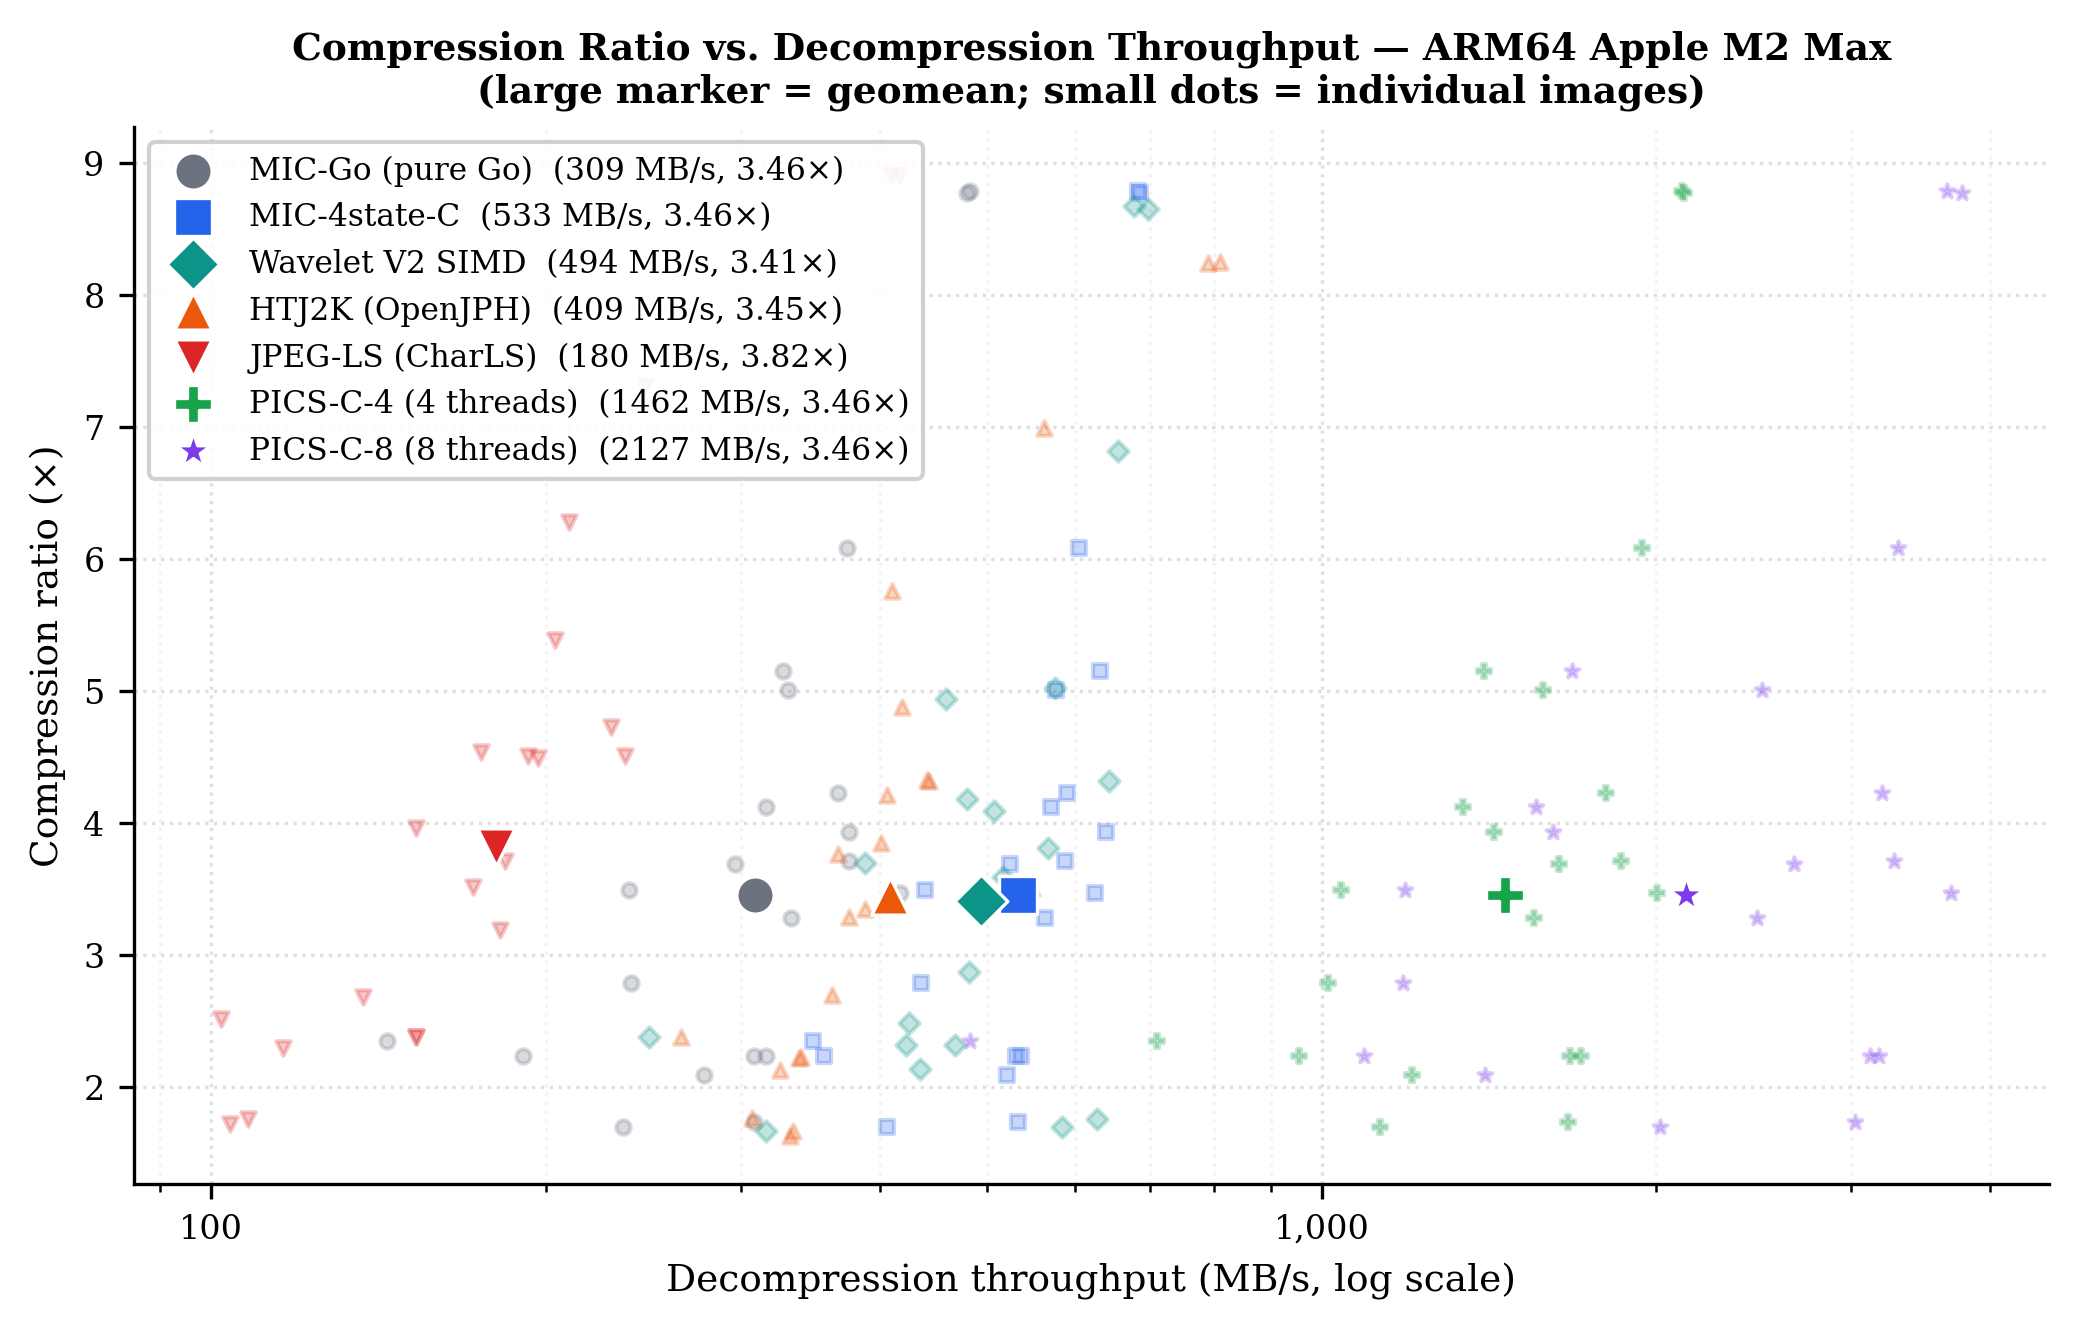
\includegraphics[width=\columnwidth]{figures/fig4_pareto.png}
\caption{Ratio vs.\ decompression throughput on ARM64. Small dots are
per-image; large markers are geometric means. MIC and JPEG-LS occupy
the Pareto frontier; HTJ2K and $\Delta$+Zstd-19 are dominated on both
axes.}
\label{fig:pareto}
\end{figure}

\textbf{Use-case decision matrix.}
Pareto analysis is limited to two quantitative axes. Real deployment
choices also depend on which CPU architectures and runtime environments
a codec covers, and on the friction of integrating it into a product
build. Table~\ref{tab:decision-matrix} normalises seven criteria so
that the best codec on each row scores~1.0; weighted sums for three
representative scenarios are reported in the final three rows. The
quantitative rows are derived from the geometric means in
Tables~\ref{tab:ratios}, \ref{tab:enc}, and
\ref{tab:decomp}; the platform and deployment rows use the rubric
in the table caption.

\begin{table}[t]
\centering
\caption{Codec selection matrix. Each criterion is normalised so the
best codec on that row scores~1.00. Quantitative rows are geometric
means across the 21-image set. AMD64 / ARM64 native rows score~1.00
when a production-grade native binary is available for that platform.
Browser compatibility: shipped purpose-built JS or WASM decoder used in
production~=~1.00; WASM port of the native library available and used in
clinical viewers (OpenJPH-JS, charls-js via Cornerstone)~=~0.85;
no browser path~=~0.0. Deployment ease: zero external runtime
dependencies~=~1.00; ubiquitous system dependency (e.g.\ libzstd)~=~0.90;
C/C++ library requiring CMake build and link integration~=~0.70.
Weight columns $w_P$, $w_A$, $w_B$ reflect typical priorities for
(P)~PACS viewer / low-latency decode, (A)~archival storage,
(B)~browser delivery.}
\label{tab:decision-matrix}
\scriptsize
\setlength{\tabcolsep}{3pt}
\begin{tabular}{lrrrrrr}
\toprule
Criterion & $w_P$ & $w_A$ & $w_B$ & MIC & HTJ2K & JPEG-LS \\
\midrule
Compression ratio                & 0.20 & 0.50 & 0.10 & 0.91 & 0.90 & \textbf{1.00} \\
Decompression throughput (ARM64) & 0.30 & 0.10 & 0.15 & \textbf{1.00} & 0.58 & 0.34 \\
Encoding throughput (ARM64)      & 0.05 & 0.10 & 0.05 & \textbf{1.00} & 0.36 & 0.22 \\
AMD64 native                     & 0.10 & 0.05 & 0.05 & \textbf{1.00} & \textbf{1.00} & \textbf{1.00} \\
ARM64 native                     & 0.10 & 0.05 & 0.05 & \textbf{1.00} & \textbf{1.00} & \textbf{1.00} \\
Browser compatibility            & 0.05 & 0.00 & 0.40 & \textbf{1.00} & 0.85 & 0.85 \\
Deployment ease                  & 0.20 & 0.20 & 0.20 & \textbf{1.00} & 0.70 & 0.70 \\
\midrule
\textbf{Weighted score (P) viewer}   & --- & --- & --- & \textbf{0.98} & 0.75 & 0.70 \\
\textbf{Weighted score (A) archival} & --- & --- & --- & \textbf{0.96} & 0.78 & 0.80 \\
\textbf{Weighted score (B) browser}  & --- & --- & --- & \textbf{0.99} & 0.78 & 0.74 \\
\bottomrule
\end{tabular}
\end{table}

\textbf{Interpretation.}
All three codecs reach parity on native AMD64 and ARM64 availability;
those rows confirm the baseline but do not differentiate the codecs.
Differentiation comes from the four quantitative rows plus browser
support and deployment friction. MIC achieves the highest weighted
score in all three scenarios under these neutral weights: 0.98 versus
0.75/0.70 for the viewer, 0.96 versus 0.78/0.80 for archival, and 0.99
versus 0.78/0.74 for browser delivery. The gap narrows on archival,
where the ratio weight rises to 0.50 and JPEG-LS edges past HTJ2K
(0.80~vs.\ 0.78) on the strength of its top compression ratio; JPEG-LS
still does not overtake MIC because its decode throughput remains
roughly $3\times$ slower even when ratio is the dominant criterion.
HTJ2K is never the highest-scoring choice under these weights, but
remains the default whenever DICOM transfer-syntax compatibility is a
hard constraint not modelled in the matrix; in such cases the matrix
serves to quantify the cost of that compatibility requirement rather
than to recommend a different codec. Practitioners with different
priorities can re-evaluate Table~\ref{tab:decision-matrix} by adjusting
$w_P$, $w_A$, or $w_B$; the per-row normalised scores remain valid
across any weighting scheme.

Future work should strengthen the evidence base with larger datasets,
shuffle-based general-purpose baselines, formal statistical reporting, and
direct browser benchmarking. Several specific items: (i) measure JPEG-LS,
$\Delta$+Zstd-19, and PICS-C-2 throughput on AMD64 so the AMD64 encoding
(Table~\ref{tab:enc}) and decoding (Table~\ref{tab:decomp})
tables are column-for-column comparable to the ARM64 tables; (ii) add a
NEON predict/update kernel for the wavelet variant on ARM64; and (iii)
extend the JavaScript decoder evaluation to the AMD64 platform.

MIC is open-source and available at
\url{https://github.com/pappuks/medical-image-codec}.

% ============================================================
\section*{Acknowledgment}

The author thanks the NEMA Working Group~4 for making the DICOM compression
sample images publicly available, and the developers of OpenJPH and CharLS for
their open-source implementations used in the comparative evaluation.

% ============================================================
\section*{Conflict of Interest}

The author declares no competing financial interests or personal relationships
that could have influenced the work reported in this paper.

% ============================================================
\section*{Data Availability}

The test images are drawn from publicly available DICOM datasets:
NEMA WG-04 compression samples~\cite{nema_wg04}, NEMA 1997~CD, and the
Clunie Breast Tomosynthesis Case~1~\cite{clunie_tomo}. The MIC implementation,
benchmark harness, and reproduction instructions are available at
\url{https://github.com/pappuks/medical-image-codec}.

% ============================================================
\IEEEtriggeratref{35}

\begin{thebibliography}{99}

\bibitem{dicom}
NEMA, ``Digital Imaging and Communications in Medicine (DICOM),''
PS3.5---Data Structures and Encoding, PS3.15---Security and System Management
Profiles,
\url{https://www.dicomstandard.org/}, 2024.

\bibitem{taubman2002}
D.\,S.\,Taubman and M.\,W.\,Marcellin,
\textit{JPEG2000: Image Compression Fundamentals, Standards and Practice}.
Springer, 2002.

\bibitem{htj2k2019}
D.\,S.\,Taubman, ``High throughput JPEG 2000 (HTJ2K): Algorithm, performance
evaluation, and potential,'' \textit{Proc.\ SPIE}, vol.\,11137, 2019.

\bibitem{loco1}
M.\,J.\,Weinberger, G.\,Seroussi, and G.\,Sapiro,
``The LOCO-I lossless image compression algorithm: Principles and
standardization into JPEG-LS,''
\textit{IEEE Trans.\ Image Process.}, vol.\,9, no.\,8, pp.\,1309--1324, 2000.

\bibitem{jpegls2}
ISO/IEC 14495-2:2003, ``Information technology---Lossless and near-lossless
compression of continuous-tone still images: Extensions---Part~2,'' 2003.

\bibitem{jpegxl}
J.\,Alakuijala \textit{et al.},
``JPEG XL next-generation image compression architecture and coding tools,''
\textit{Proc.\ SPIE 11137}, Sep.\,2019.

\bibitem{duda2009}
J.\,Duda, ``Asymmetric numeral systems,'' arXiv:0902.0271, 2009.

\bibitem{duda2013}
J.\,Duda, ``Asymmetric numeral systems: entropy coding combining speed of
Huffman coding with compression rate of arithmetic coding,''
arXiv:1311.2540, 2013.

\bibitem{fse}
Y.\,Collet, ``Finite State Entropy---A new breed of entropy coder,''
\url{https://github.com/Cyan4973/FiniteStateEntropy}, 2013.

\bibitem{rfc8878}
Y.\,Collet and M.\,Kucherawy,
``Zstandard Compression and the `application/zstd' Media Type,''
RFC~8878, IETF, Feb.\,2021.


\bibitem{mahapatra2007}
S.\,Mahapatra and K.\,Singh,
``An FPGA-based implementation of multi-alphabet arithmetic coding,''
\textit{IEEE Trans.\ Circuits Syst.\ I}, vol.\,54, no.\,8, pp.\,1678--1686,
2007.

\bibitem{kosolobov2022}
D.\,Kosolobov, ``Efficiency of ANS Entropy Encoders,''
arXiv:2201.02514, 2022.

\bibitem{bamler2022}
R.\,Bamler, ``Understanding Entropy Coding With Asymmetric Numeral Systems
(ANS): a Statistician's Perspective,'' arXiv:2201.01741, 2022.

\bibitem{giesen2014}
F.\,Giesen, ``Interleaved entropy coders,'' arXiv:1402.3392, 2014.

\bibitem{giesen2014b}
F.\,Giesen, ``ryg\_rans: Public domain rANS encoder/decoder,''
\url{https://github.com/rygorous/ryg_rans}, 2014.

\bibitem{lin2023}
F.\,Lin, K.\,Arunruangsirilert, H.\,Sun, and J.\,Katto,
``Recoil: Parallel rANS Decoding with Decoder-Adaptive Scalability,''
\textit{Proc.\ 52nd ICPP '23}, pp.\,31--40, 2023.

\bibitem{weissenberger2019}
A.\,Weissenberger and B.\,Schmidt,
``Massively Parallel ANS Decoding on GPUs,''
\textit{Proc.\ 48th ICPP '19}, Article~100, 2019.

\bibitem{wu1997}
X.\,Wu and N.\,Memon,
``Context-based, adaptive, lossless image coding,''
\textit{IEEE Trans.\ Commun.}, vol.\,45, no.\,4, pp.\,437--444, 1997.

\bibitem{sneyers2016}
J.\,Sneyers and P.\,Wuille,
``FLIF: Free Lossless Image Format based on MANIAC Compression,''
\textit{Proc.\ IEEE ICIP}, 2016.

\bibitem{legall1988}
D.\,Le Gall and A.\,Tabatabai,
``Sub-band coding of digital images using symmetric short kernel filters and
arithmetic coding techniques,'' \textit{Proc.\ IEEE ICASSP}, pp.\,761--764,
1988.

\bibitem{sweldens1996}
W.\,Sweldens,
``The Lifting Scheme: A custom-design construction of biorthogonal wavelets,''
\textit{Appl.\ Comput.\ Harmon.\ Anal.}, vol.\,3, no.\,2, pp.\,186--200, 1996.

\bibitem{daubechies1998}
I.\,Daubechies and W.\,Sweldens,
``Factoring wavelet transforms into lifting steps,''
\textit{J.\ Fourier Anal.\ Appl.}, vol.\,4, no.\,3, pp.\,247--269, 1998.

\bibitem{calderbank1998}
A.\,R.\,Calderbank, I.\,Daubechies, W.\,Sweldens, and B.-L.\,Yeo,
``Wavelet transforms that map integers to integers,''
\textit{Appl.\ Comput.\ Harmon.\ Anal.}, vol.\,5, no.\,3, pp.\,332--369, 1998.


\bibitem{liu2017}
F.\,Liu \textit{et al.},
``The Current Role of Image Compression Standards in Medical Imaging,''
\textit{Information}, vol.\,8, no.\,4, p.\,131, Oct.\,2017.

\bibitem{clunie2000}
D.\,A.\,Clunie,
``Lossless Compression of Grayscale Medical Images: Effectiveness of
Traditional and State-of-the-Art Approaches,''
\textit{Proc.\ SPIE Medical Imaging}, 2000.

\bibitem{png}
W3C, ``Portable Network Graphics (PNG) Specification (Second Edition),''
ISO/IEC 15948:2003, Nov.\,2003.

\bibitem{taubman2022}
D.\,Taubman, A.\,Naman, M.\,Smith, P.-A.\,Lemieux, H.\,Saadat, O.\,Watanabe,
and R.\,Mathew,
``High Throughput JPEG~2000 for Video Content Production and Delivery Over IP
Networks,''
\textit{Front.\ Signal Process.}, vol.\,2, Article 885644, Apr.\,2022.

\bibitem{williams2009}
S.\,Williams, A.\,Waterman, and D.\,Patterson,
``Roofline: An insightful visual performance model for multicore
architectures,''
\textit{Commun.\ ACM}, vol.\,52, no.\,4, pp.\,65--76, Apr.\,2009.

\bibitem{openjph}
A.\,N.\,Aous,
``OpenJPH: An open-source implementation of High-Throughput JPEG~2000,''
\url{https://github.com/aous72/OpenJPH}, 2024.

\bibitem{charls}
Team CharLS,
``CharLS: A C/C++ JPEG-LS library implementation,''
\url{https://github.com/team-charls/charls}, 2024.

\bibitem{nema_wg04}
NEMA Working Group~4 (WG-04),
``DICOM Compression Sample Images,''
National Electrical Manufacturers Association,
\url{https://www.dicomstandard.org/Resources/Open-Content/Compression-Samples},
2024.

\bibitem{clunie_tomo}
D.\,A.\,Clunie,
``Breast Tomosynthesis Case~1,'' DICOM sample images,
\url{http://www.dclunie.com/pixelmedimagecases/tomo/case1/}, 2009.

\bibitem{geldreich_pareto}
R.\,Geldreich, ``Quick survey of the lossless decompression Pareto frontier,''
2015, \url{http://richg42.blogspot.com/2015/11/the-lossless-decompression-pareto.html}.

\bibitem{jpegxl_pareto}
J.\,Sneyers, ``JPEG XL and the Pareto front,'' Cloudinary Blog, 2022,
\url{https://cloudinary.com/blog/jpeg-xl-and-the-pareto-front}.

\bibitem{fcbench}
J.\,Tao \textit{et al.}, ``FCBench: Cross-domain benchmarking of lossless
compression,'' \textit{Proc.\ VLDB Endowment}, vol.\,17, no.\,7,
pp.\,1418--1431, 2024.

\bibitem{lossless_unified_score}
A.\,Anonymous, ``Challenges and solutions in selecting optimal lossless data
compression algorithms,'' arXiv:2509.25219, 2025.

\bibitem{saaty_ahp}
T.\,L.\,Saaty, \textit{The Analytic Hierarchy Process: Planning, Priority
Setting, Resource Allocation}. New York, NY, USA: McGraw-Hill, 1980.

\bibitem{clunie_miit2009}
D.\,A.\,Clunie, ``DICOM support for compression: More than JPEG,''
\textit{Medical Imaging Informatics and Teleradiology (MIIT)}, 2009,
\url{https://www.dclunie.com/papers/MIIT_2009_DicomCompression_Clunie.pdf}.

\bibitem{sayood}
K.\,Sayood, \textit{Introduction to Data Compression}, 5th ed.
Burlington, MA, USA: Morgan Kaufmann, 2017.

\end{thebibliography}

\end{document}
